 \documentclass{article}

\title{StochAn}
\author{mishamilovidov}
\date{December 2025}

\usepackage{a4wide}
\usepackage[utf8]{inputenc}
\usepackage[russian]{babel}
\usepackage{graphicx}
\usepackage{amsmath}
\usepackage{float}
\usepackage{hyperref}
\usepackage{amssymb}
\usepackage{bbm}
\usepackage{amsthm}
\usepackage{indentfirst}
\usepackage{float}
\usepackage{comment}
\usepackage{subcaption}
\usepackage[thinc]{esdiff}

\DeclareMathOperator{\sinc}{sinc}
%\DeclareMathOperator{\arctg}{arctg}
\DeclareMathOperator{\sgn}{sgn}
\DeclareMathOperator{\const}{const}
\DeclareMathOperator{\grad}{grad}
\renewcommand{\le}{\leqslant}
\renewcommand{\ge}{\geqslant}
\newcommand{\scalar}[2]{\left<#1,#2\right>}
\newcommand{\norm}[1]{\left\lVert #1 \right\rVert}
\newcommand{\abs}[1]{\left\lvert #1 \right\rvert}

\renewcommand{\labelenumii}{\arabic{enumi}.\arabic{enumii}}
\renewcommand{\labelenumiii}{\arabic{enumi}.\arabic{enumii}.\arabic{enumiii}}
\renewcommand{\labelenumiv}{\arabic{enumi}.\arabic{enumii}.\arabic{enumiii}.\arabic{enumiv}}

\newtheorem{theorem}{Теорема}
\newtheorem{statement}{Утверждение}
\newtheorem*{remark}{Замечание}
\theoremstyle{definition}
\newtheorem{definition}{Определение}[section]

\begin{document}

\thispagestyle{empty}

\begin{center}
\ \vspace{-3cm}


\includegraphics[width=0.5\textwidth]{data/msu.eps}\\
{\scshape Московский государственный университет имени М.~В.~Ломоносова}\\
Факультет вычислительной математики и кибернетики\\
Кафедра системного анализа

\vfill

{\LARGE Практикум по курсу}

\vspace{1cm}

{\Huge\bfseries <<Стохастический анализ и моделирование>>}
\end{center}

\vspace{1cm}

\begin{flushright}
  \large
  \textit{Студент 415 группы}\\
  М.\,В.~Миловидов

  \vspace{5mm}

  \textit{Руководитель практикума}\\
  В.\,А.~Сливинский
\end{flushright}

\vfill

\begin{center}
Москва, 2025
\end{center}
\newpage

\section{Задание 1}

\subsection{Постановка задачи}
\begin{enumerate}
    \item Реализовать генератор схемы Бернулли с заданной вероятностью успеха \(p\). На
основе генератора схемы Бернулли построить датчик биномиального распреде-
ления.
    \item Реализовать генератор геометрического распределения; проверить для данного
распределения свойство отсутствия памяти.
    \item Промоделировать игру в орлянку: бесконечную последовательность независимых испытаний Бернулли с бросанием “правильной” (честной, \(p = 0.5\)) монеты.
Величина “выигрыша” \(S_n\) определяется как сумма по n испытаниям значений \(1\)
и \(-1\) в зависимости от выпавшей стороны монеты. Проиллюстрировать в виде
ломаной поведение нормированной суммы \(Y(i) = \frac{S_i}{\sqrt{n}}\) как функцию от номера
испытания \(i\) для отдельно взятой траектории. Дать теоретическую оценку для
значения \(Y(n)\) при \(n \to \infty\)
\end{enumerate}

\subsection{Теоретические сведения}

\subsubsection{Схема Бернулли и биномиальное распределение}

Схемой Бернулли с заданной вероятностью \(p\) называется эксперимент,
состоящий из серии испытаний, удовлетворяющих следующим условиям:
\begin{itemize}
    \item Отсутствие взаимного влияния в испытаниях;
    \item Воспроизводимость. Однородные испытания проводятся в сходных (не обязательно идентичных) условиях;
    \item Существует признак, который реализуется (“успех” с вероятностью \(p\)) или не
реализуется (“неуспех” с вероятностью \(q = (1 − p)\)) в испытании. Признак может
быть отнесен к любому из испытаний (в силу их однородности).
\end{itemize}
Здесь и далее, под генератором и датчиком подразумевается функция, возвращающая выборку заданного размера из соответствующего распределения.

Распределение Бернулли задается следующим образом:
\[X \sim \text{Ber}(p)\ (p \in [0, 1]) \Leftrightarrow \mathbb{P}(X = k) = \begin{cases}
      1-p,&k = 0\\
      p,&k = 1\\
  \end{cases}\]
Биномиальное распределение определяется как число успехов в \(n\) испытаниях Бернулли:
\[X \sim \text{Bin}(n, p)\ (n \in \mathbb{N},\ p \in [0, 1]) \Leftrightarrow \mathbb{P}(x = k) = C_n^k p^k (1 - p)^{n - k},\ k \in \overline{0, n}.\]

\subsubsection{Геометрическое распределение}

Функция вероятности геометрического распределения имеет вид $\mathbb{P}(X = n) = p(1 - p)^n$. Получим геометрическое распределение через экспоненциальное. Пусть $\xi \sim exp(\lambda)$, тогда $\lfloor \xi \rfloor \sim Geom(p)$, где $p = 1 - e^{-\lambda}$.
Покажем, что это так. Функция распределения имеет вид $F_\xi(x) = 1-e^{-\lambda x}$. Поэтому для $n \in \mathbb{N}_0$
$$
    \mathbb{P}(\lfloor \xi \rfloor = n) = \mathbb{P}(n \le \xi \le n + 1) = e^{-n\lambda} (1 - e^{-\lambda}) = (1 - p)^np
$$
Таким образом, моделирование геометрическое распределения с параметром p сводится к моделированию экспоненциального распределения с параметром $\lambda = - \ln(1 - p)$.
Воспользуемся методом обращения функции распределения:
$$
    F_\xi^{-1}(y) = -\frac{1}{\lambda}\ln(1 - y)
$$
Пусть случайная величина $\xi$ имеет непрерывную и строго возрастающую функцию распределения $F_\xi$. Тогда $F_\xi^{-1}(U) \sim \xi,\ U \sim \mathcal{U}(0, 1)$
$$
    \mathbb{P}(F_\xi^{-1}(U) < x) = \mathbb{P}(U < F_\xi(x)) = F_\xi(x),
$$
поэтому $F_\xi^{-1}(U) \sim \xi.$

Распределение дискретной случайной величины X обладает свойством отсутствия памяти, если $\mathbb{P}(X > t + \tau |X \ge \tau) = \mathbb{P}(X > t)\ \forall t, \tau \in \mathbb{Z},\, t > 0$.
Для геометрического распределения $\mathbb{P}(X > t) = (1 - p)^{t + 1}$ и
$$
    \mathbb{P}(X > t + \tau |X \ge \tau) = \frac{\mathbb{P}(X > t + \tau,\, X \ge \tau)}{\mathbb{P}(X \ge \tau)} = \frac{(1 - p)^{t + \tau + 1}}{(1 - p)^{\tau}} = (X > t).
$$
Следовательно, геометрическое распределение обладает свойством отсутствия памяти.

\subsubsection{Игра в орлянку}

Игра в орлянку --- бесконечная последовательность независимых испытаний с бросанием правильной монеты. Выйгрыш $S_n$ определяется как сумма по n испытаниям значений 1 и -1 в значении от выпавшей стороны.

Теоретическую оценку можно дать, используя центральную предельную теорему (ЦПТ). Она говорит, что если $\{X_i\}$ --- последовательность независимых одинаконово распределенных случайных величин с матожиданием $\mu$ и дисперсией $\sigma^2$, то
$$
    \frac{S_n - \mu n}{\sigma \sqrt n} \xrightarrow[n → \infty]{d} \mathcal{N}(0, 1),
$$
где $\mathcal{N}(0, 1)$ --- стандартное нормальное распределение.
В данном случае $\mu = 0,\, \sigma = 1$ и $Y(n) = \frac{S_n}{\sqrt n} \xrightarrow[n \rightarrow \infty]{d} \mathcal{N}(0, 1)$.

\subsection{Результаты работы программы}

\subsubsection{Схема Бернулли и биномиальное распределение}

Сгенерируем выборку из биномиального распределения размера 1000 с параметрами \(p = 0.5,\, n = 10\):

\begin{figure}[H]
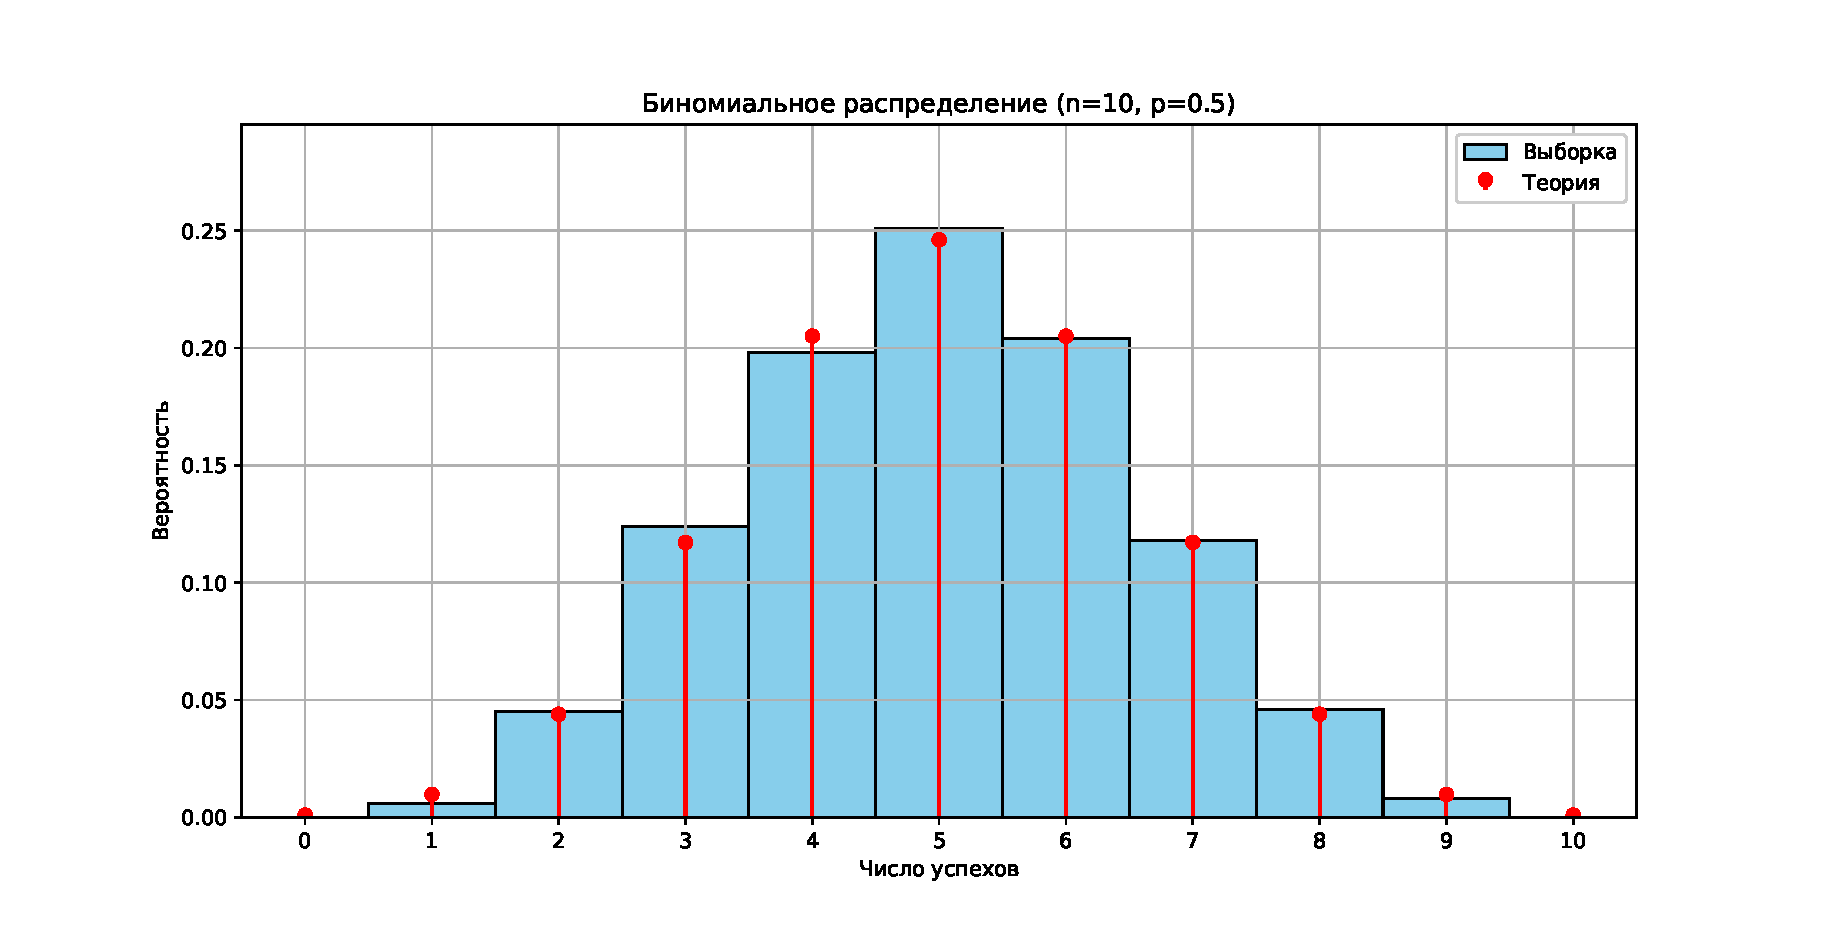
\includegraphics[width=1\textwidth]{data/ex1/bin.eps}
\label{fig:ex1/bin}
\end{figure}

\subsubsection{Геометрическое распределение}

Сгенерируем выборку из геометрического распределения размера 1000 с параметром \(p = 0.5\):

\begin{figure}[H]
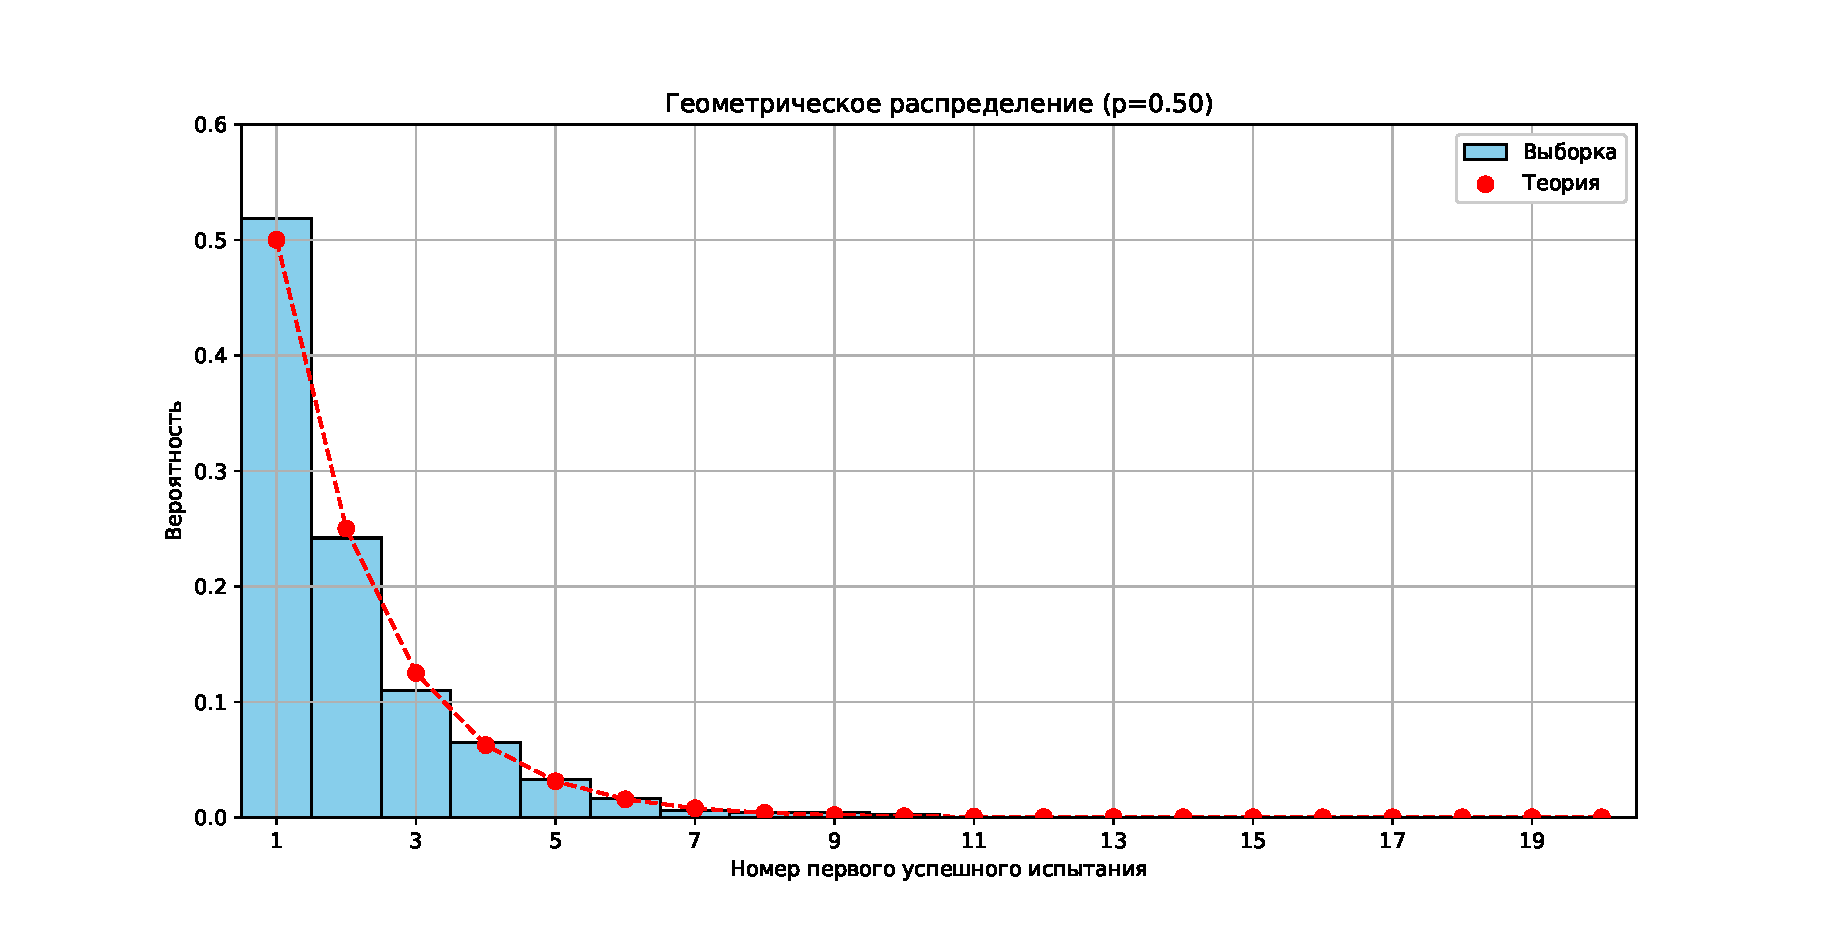
\includegraphics[width=1\textwidth]{data/ex1/geom.eps}
\label{fig:ex1/geom}
\end{figure}

\subsubsection{Игра в орлянку}

Проиллюстрируем поведение величины $Y(i) = \frac{S_i}{\sqrt n}$ как функцию номера испытания $i = 1, \dots ,n$ для отдельно взятой траектории:

\begin{figure}[H]
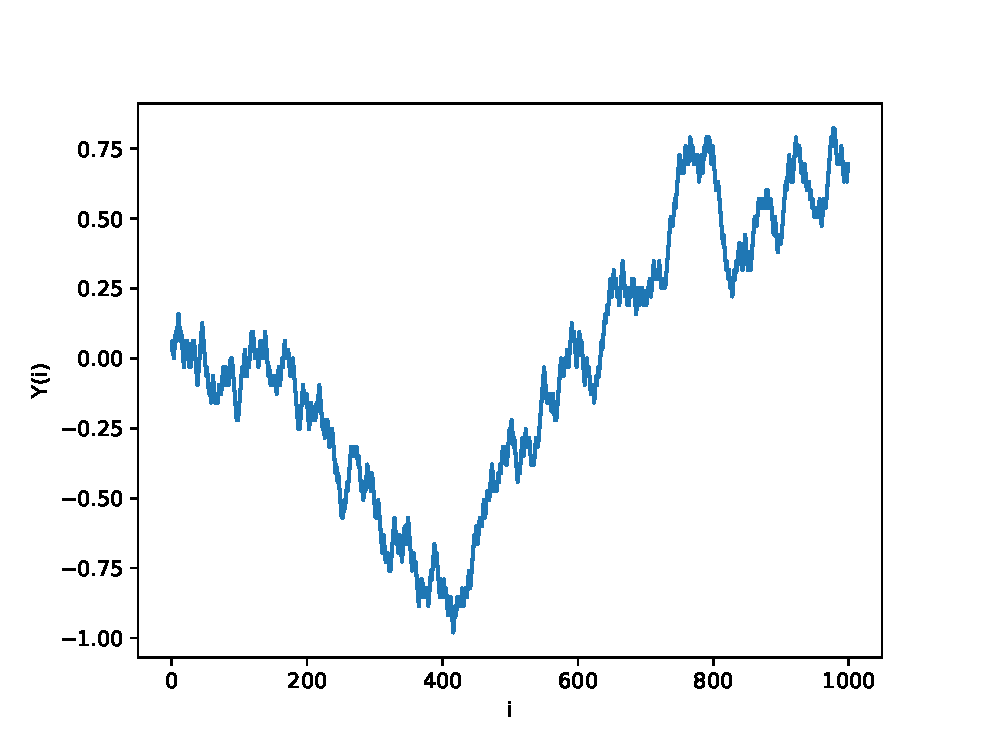
\includegraphics[width=1\textwidth]{data/ex1/or1.eps}
\label{fig:ex1/or1}
\caption{Симуляция величины \(Y(i)\)}
\end{figure}

Рассмотрим распределение данной случайной величины после 1000 итераций:

\begin{figure}[H]
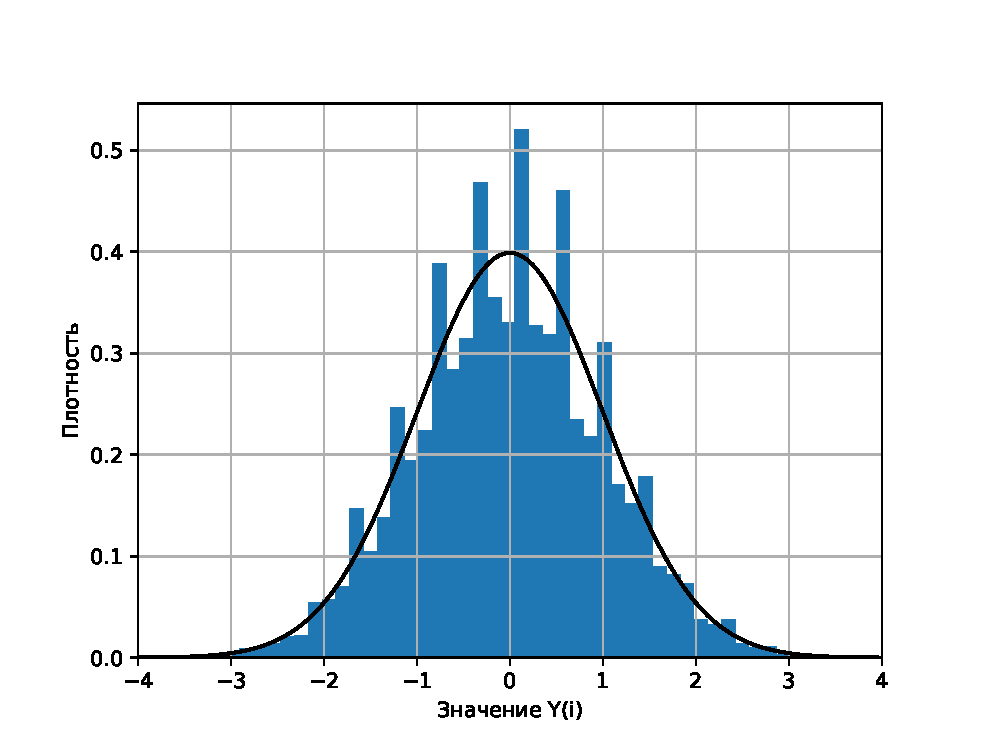
\includegraphics[width=1\textwidth]{data/ex1/or2.eps}
\label{fig:ex1/or2}
\caption{Распределение величины \(Y(1000)\) (10000 симуляций).}
\end{figure}

Как видно, выборочная плотность распределения близка к плотности нормального распределения.



\section{Задание 2}
\subsection{Постановка задачи}
\begin{enumerate}
    \item Построить датчик сингулярного распределения, имеющий в качестве функции
распределения канторову лестницу. С помощью критерия Колмогорова убедиться в корректности работы датчика.
    \item Для канторовых случайных величин с помощью критерия Смирнова проверить
свойство симметричности относительно \(\frac{1}{2}\) (\(X\) и \(1 − X\) распределены одинаково)
и свойство самоподобия относительно деления на 3 (условное распределение \(Y\)
при условии \(Y \in [0, 1/3]\) совпадает с распределением \(\frac{Y}{3}\)).
    \item Рассчитать значения математического ожидания и дисперсии для данного распределения. Сравнить теоретические значения с эмпирическими (для различных объемов выборок), проиллюстрировать сходимость эмпирических значений
к теоретическим.
\end{enumerate}

\subsection{Теоретические сведения}

\subsubsection{Сингулярное распределение}
Построим датчик сингулярного распределения, имеющий в качестве функции распределения канторову лестницу. Заметим, что из определения канторовой лестницы следует, что каждая цифра в троичной записи значения случайной величины равна 0 или 2 с вероятностью $\frac{1}{2}$. Его можно представить в виде $\alpha_1 \frac{1}{3} + \alpha_2 \frac{1}{9} + \dots \ $, где $\alpha_i \in \{0, 2\}$. Таким образом, будем использовать датчик распределения Бернулли и считать данную сумму до 20 члена (это даст достаточную точность).
\subsubsection{Проверка по критерию Колмогорова}
Проверим корректность при помощи критерия Колмогорова. Установим уровень значимости $\alpha$ = 0.05. Пусть $D_n = \sup_x \lvert F_n(x) - F(x) \rvert$, где $F_n$ и $F$ --- эмпирическая и истинная функции распределения. Если мы получим p-value для статистики $\sqrt n D_n$ и распределения Колмогорова большее $\alpha$, то нулевая гипотеза о том, что полученная выборка подчиняется распределению, имеющему в качестве функции распределения канторову лестницу, принимается. Иначе она отвергается. p-value имеет смысл вероятности получить более экстремальную статистику, чем наблюдаемую. Если оно мало, значит значение статистики маловероятно при нулевой гипотезе, значит ее стоит отвергнуть.

\subsubsection{Проверка по критерию Смирнова}
Будем проверять симметричность относительно $\frac{1}{2}$ ($X$ и $1 - X$ распределены одинаково) и свойство самоподобия относительно деления на 3 (условное распределение $Y$ при условии $Y \in [0, \frac{1}{3}]$ совпадает с распределением $\frac{Y}{3}$). Для этого используем критерий Смирнова, который используется для проверки гипотезы о принадлежности двух независимых выборок одному закону распределения. Пусть $F_{1, n},\, F_{2, m}$ --- выборочные функции распределения, построенные по независимым выборкам объема $n$ и $m$, $D_{n, m} = \sup_x \lvert F_{1, n} - F_{2, m} \rvert$ Критерий Смирнова гласит, что если статистика $\sqrt{\frac{nm}{n + m}}D_{n, m}$ превышает квантиль распределения Колмогорова $K_{\alpha}$ для заданного уровня значимости $\alpha$, то нулевая гипотеза $H_0$ об однородности выборок отвергается. Иначе она принимается на уровне $\alpha$. Выберем $\alpha = 0.05$. Возьмем одинаковый размер выборок N, посчитаем статистику и найдем значение функции распределения Колмогорова.

\subsubsection{Рассчет матожидания и дисперсии}

Посчитаем теоретические и эмпирические значения матожидания и дисперсии. Используем то, что случайная величина, имеющая функцию распределения Кантора, представима в виде
$$X = \sum_{n = 1}^\infty \alpha_i\frac{2}{3^n},$$
где $\alpha_i$ имеют распределение Бернулли с параметром 0.5. Тогда
$$\mathbb{E}X = \mathbb{E}\sum_{n = 1}^\infty \alpha_i\frac{2}{3^n} = \sum_{n = 1}^\infty \frac{2}{3^n}\mathbb{E}\alpha_i = \sum_{n = 1}^\infty \frac{1}{3^n} = \frac{1}{3}\frac{1}{1-\frac{1}{3}} = \frac{1}{2}$$
$$\mathbb{D}X = \mathbb{D}\sum_{n = 1}^\infty \alpha_i\frac{2}{3^n} = \sum_{n = 1}^\infty\frac{4}{9^n}\mathbb{D}\alpha_i = \sum_{n = 1}^\infty\frac{1}{9^n} = \frac{1}{9}\frac{1}{1-\frac{1}{9}} = \frac{1}{8}$$

\subsection{Результаты работы программы}

\subsubsection{Сингулярное распределение}
Сгенерируем 1000 случайных величин из датчика сингулярного распределения, построим по ним выборочную функцию распределения и сравним с истинной (функция Кантора):

\begin{figure}[H]
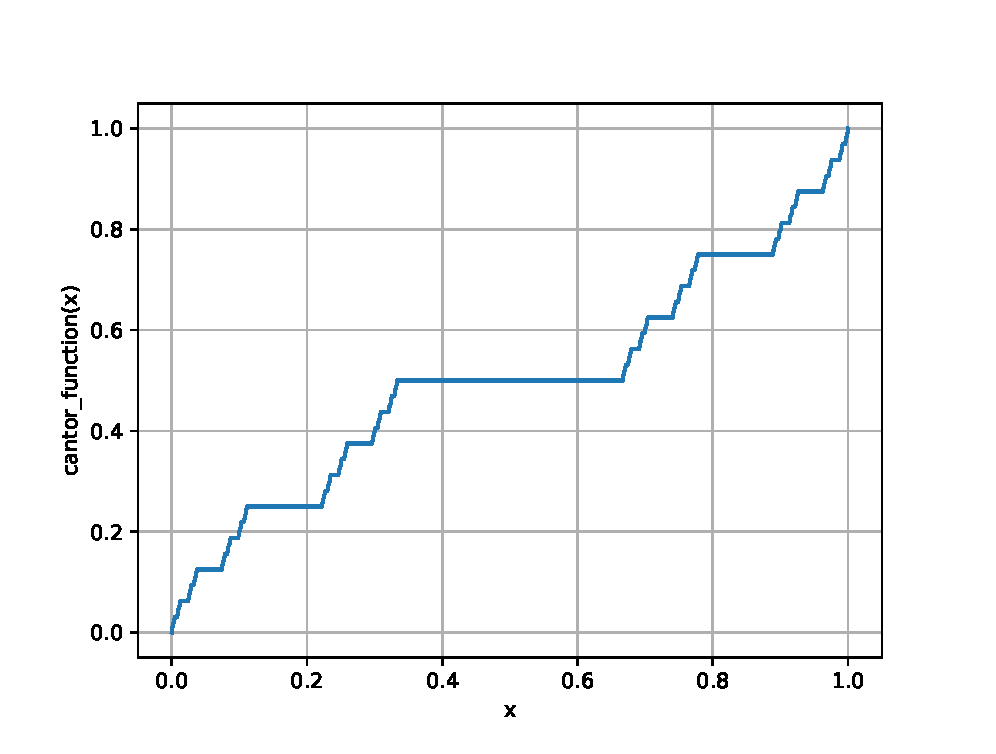
\includegraphics[width=0.5\textwidth]{data/ex2/true_cantor.eps}
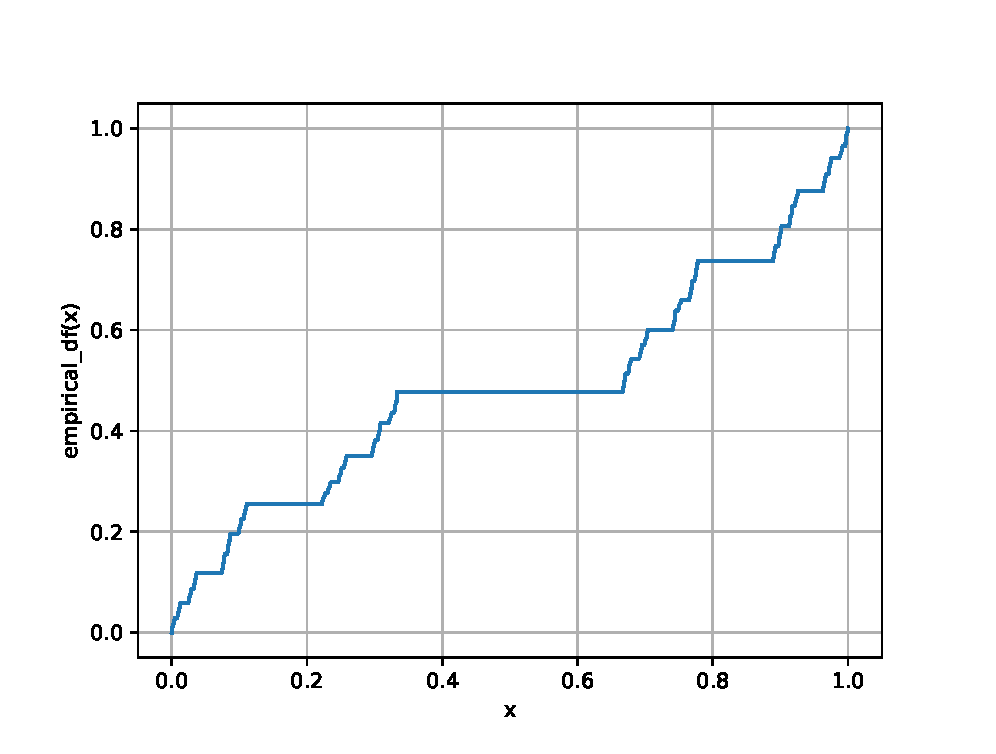
\includegraphics[width=0.5\textwidth]{data/ex2/empirical_cantor.eps}
\label{fig:ex2/cantor}
\caption{Истинная и эмпирическая функции распределения}
\end{figure}


\subsubsection{Проверка по критерию Колмогорова}
Проведем 1000 испытаний и посмотрим, в какой доле случаев полученное p-value меньше заданного уровня значимости \(\alpha = 0.05\). Будем генерировать выборку размера 1000. 

В результате работы программы получаем, что гипотеза отклоняется в 4.1\% случаев, что является достаточно хорошим результатом. 

\subsubsection{Проверка по критерию Смирнова}

Проведем аналогичную процедуру для критерия Смирнова. Получим, что гипотеза отклоняется в 4\% случаев. Таким образом, критерии дают очень похожий результат для данного распределения.

\subsubsection{Рассчет матожидания и дисперсии}

Проведя вычисления для выборки размера 10000, получим, что выборочное матожидание равно 0.4948125064453071, а выборочная дисперсия --- 0.12508305064606734, что очень близко к теоретическим значениям. Проиллюстрируем сходимость эмпирических значений к теоретическим при стремлении размера выборки к бесконечности:

\begin{figure}[H]
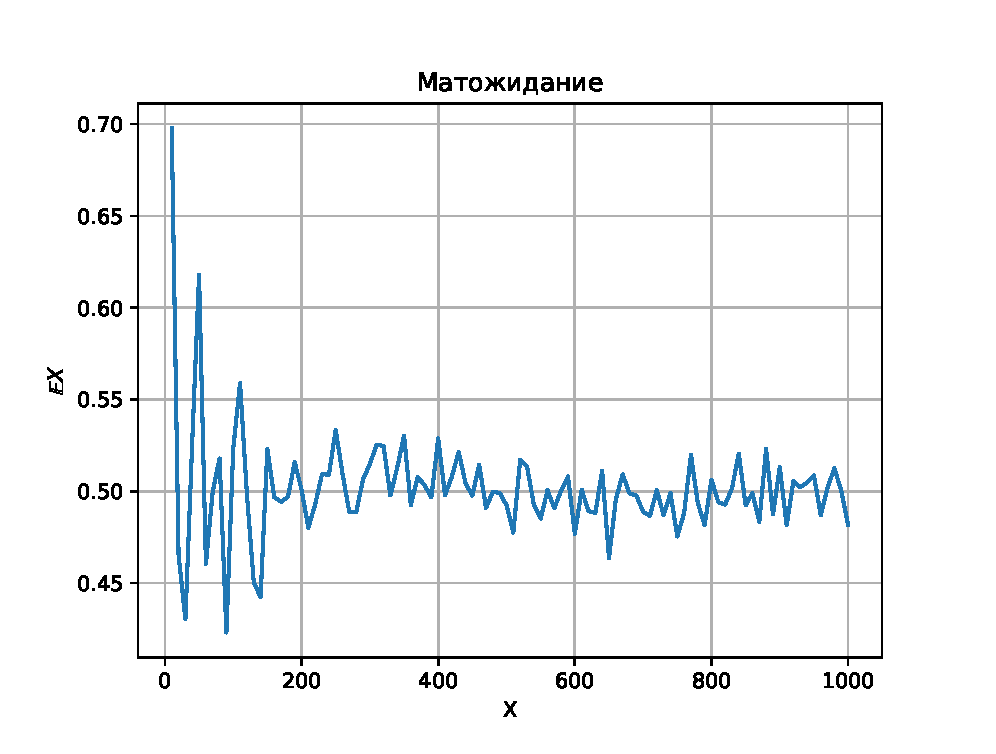
\includegraphics[width=0.5\textwidth]{data/ex2/ME.eps}
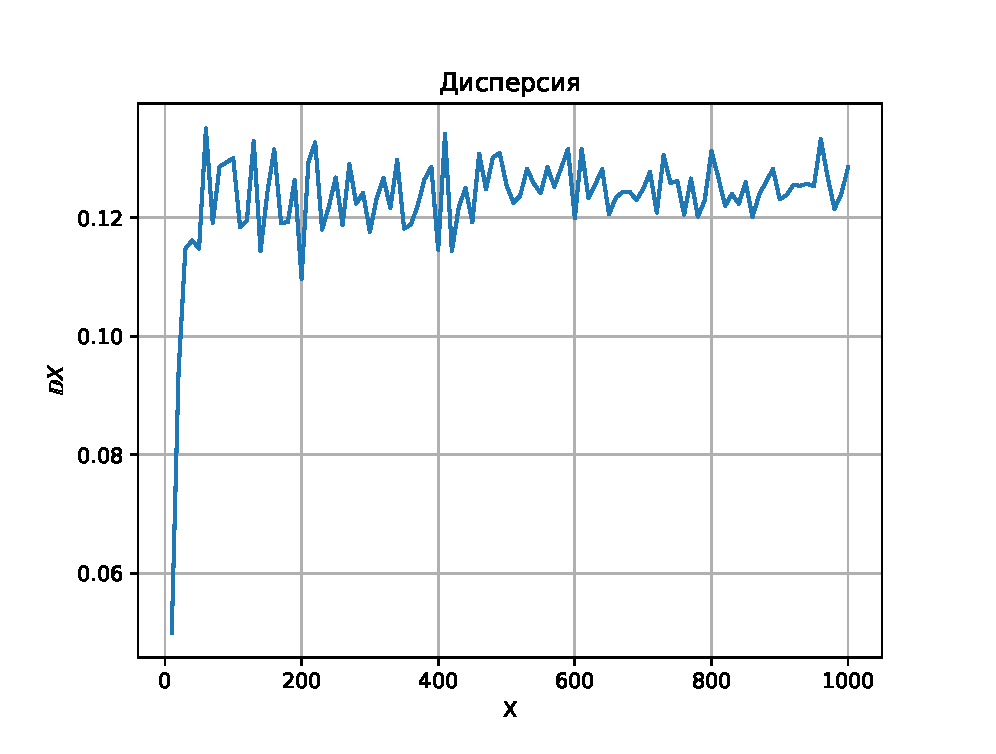
\includegraphics[width=0.5\textwidth]{data/ex2/disp.eps}
\caption{Выборочные матожидание и дисперсия}
\label{fig:ex2/ME_disp}
\end{figure}

Видно, что обе величины сходятся к теоретическому значению.


\section{Задание 3}
\subsection{Постановка задачи}
\begin{enumerate}
    \item Построить датчик экспоненциального распределения. Проверить для данного
распределения свойство остутствия памяти.
\item Пусть \(X_1, \dots, X_n\) --- независимые экспоненциально распределенные случайные
величины с параметрами \(\lambda_1,\dots,\lambda_n\). Найти распределение случайной величины
\(Y = \min(X_1,\dots,X_n)\).
\item На основе датчика экспоненциального распределения построить датчик пуассоновского распределения.
\item Построить датчик пуассоновского распределения как предел биномиального распределения. Убедиться в корректности построенного датчика при помощи критерия \(\chi^2\) Пирсона.
\item Построить датчик стандартного нормального распределения методом моделирования случайных величин парами с переходом в полярные координаты (преобразование Бокса-Мюллера). Проверить при помощи t-критерия Стьюдента равенство математических ожиданий, а при помощи критерия Фишера — равенство
дисперсий.

\end{enumerate}

\subsection{Теоретические сведения}

\subsubsection{Датчик экспоненциального распределения}

Датчик экспоненциального распределения был получен в задаче 1 путем обращения функции распределения.

Проверим для данного распределения свойство отсутствия памяти. Распределение дискретной случайной величины X обладает свойством отсутствия памяти, если $$(X > t + \tau |X \ge \tau) = (X > t)\ \forall t, \tau \in \mathbb{Z},\, t > 0.$$
В нашем случае
$$\mathbb{P}(X > t + \tau |X \ge \tau) = \frac{\mathbb{P}(X > t + \tau,\, X \ge \tau)}{\mathbb{P}(X \ge \tau)} = \frac{\mathbb{P}(X > t + \tau)}{\mathbb{P}(X \ge \tau)} = \frac{e^{-\lambda(t + \tau)}}{e^{-\lambda \tau}} = e^{-\lambda t} = \mathbb{P}(X > t)$$
Таким образом, экспоненциальное распределение обладает свойством отсутствия памяти.

\subsubsection{Распределение минимума}

Пусть $X_1, \dots, X_n$ --- независимые экспоненциально распределенные случайные величины с параметрами $(\lambda_1, \dots, \lambda_n)$. Найдем распределение случайной величины $Y = \min(X_1, \dots, X_n)$. Учитывая, что $\mathbb{P}(X > t) = e^{-\lambda t}$, получим:
$$\mathbb{P}(\min(X_1, \dots, X_n) > t) = \mathbb{P}(X_1 > t, \dots, X_n > t) = \prod_{k = 1}^n\mathbb{P}(X_k > t) = \prod_{k = 1}^n e^{-\lambda_k t} = e^{-(\lambda_1 + \ldots + \lambda_n) t}$$
Таким образом, полученная случайная величина имеет экспоненциальное распределение с параметром $\lambda = \lambda_1 + \ldots + \lambda_n$

\subsubsection{Датчик пуассоновского распределения через экспоненциальное}

Пуассоновское распределение имеет функцию вероятности $\mathbb{P}(Y = k) = \frac{\lambda^k}{k!}e^{-\lambda}$. Будем использовать пуассоновский случайный процесс $N(t) \sim Pois(\lambda t)$. Для него можно определить случайную величину $\tau$, равную времени между событиями, то есть изменениями значения $N(t)$. Известно, что $\tau \sim Exp(\lambda)$. При $t = 1\ N(1) \sim Pois(\lambda)$. Будем генерировать случайные величины $\tau$ и суммировать их до того, пока сумма не превысит 1. Посчитав число слагаемых, получим число событий за единицу времени, то есть реализацию пуассоновской случайной величины. При этом слагаемое, после которого сумма превысила 1, учитывать не нужно, так как соответствующее событие произошло уже позже $t = 1$

\subsubsection{Датчик пуассоновского распределения через биномиальное}

Биномиальное распределение с параметрами $n,\, p$ имеет функцию вероятности $\mathbb{P}(X = k) = C_n^kp^k(1-p)^{n - k}$. Положим $pn = \lambda = const$, то есть $p = \frac{\lambda}{n}$. При $n \gg k$ верно $C_n^k \approx \frac{n^k}{k!}$, $(1 - p)^{n - k} = \left(1 - \frac{\lambda}{n}\right)^{n - k} \rightarrow e^{-\lambda}$. Тогда при $n \gg k$ имеем приближенное равенство:
$$\mathbb{P}(X = k) \approx \frac{n^k}{k!}p^ke^{-\lambda} = \frac{\lambda^k}{k!}e^{-\lambda} \sim Pois(\lambda)$$

Проверим правильность при помощи критерия согласия Пирсона. В нем используется статистика хи-квадрат:
$$\chi^2 = n \sum_{i = 0}^k \frac{(\frac{n_i}{n} - \mathbb{P}_i(X))^2}{\mathbb{P}_i(X)},$$
где $n_i$ --- число значений, равных $i$, $\mathbb{P}_i(X) = \mathbb{P}(X = i)$ при $i = \overline{0,k-1}$; $n_k$ --- число значений, больших либо равных $k$, $\mathbb{P}_k(X) = \mathbb{P}(X \ge k)$. Зафиксируем уровень значимости $\alpha = 0.05$. Нулевая гипотеза о том, что выборка порождена пуассоновским распределением принимается, если значение функции распределения $\chi^2_{k-1}$ на статистике $\chi_2$ больше уровня значимости, иначе она отвергается. k выбирается так, чтобы при каждом значении $i < k$ было достаточно элементов выборки, равных $i$ (>5) (другой вариант --- выбирать интервалы, на которых достаточно значений).

\subsubsection{Датчик стандартного нормального распределения}

Воспользуемся преобразованием Бокса-Мюллера. Пусть $r$ и $\varphi$ --- независимые равномерно распределенные на отрезке [0, 1]. Тогда случайные величины
$$z_0 = \cos(2\pi \varphi)\sqrt{-2\ln r},\, z_1 = \sin(2\pi \varphi)\sqrt{-2\ln r}$$
независимы и имеют стандартное нормальное распределение. Нам понадобится только одна из них.

Проверим, что матожидание равно 0, при помощи критерия Стьюдента. Зафиксируем уровень значимости \(\alpha\) = 0.05. В критерии используется следующая статистика:
$$t = \frac{\overline X - m}{s_X/\sqrt n},$$
где $\overline X$ --- выборочное матожидание, $s_X$ --- несмещенное стандартное отклонение, $m = 0$ --- теоретическое значение матожидания. Рассматривается функция распределения Стьюдента.

В данном случае, в отличие от предыдущих, критерий является двусторонним, то есть надо проверять критические области с обеих сторон. Поэтому в данном случае берется минимум из вероятности попасть вправо или влево от статистики (и умножается на 2, т. к. вероятность попасть в каждую критическую область равна $\alpha/2$).

Проверим, что дисперсии двух выборок равны, при помощи критерия Фишера. Зафиксируем уровень значимости \(\alpha\) = 0.05. В критерии используется следующая статистика:
$$F = \frac{s^2_X}{s^2_Y},$$
где $s^2_X, s^2_Y$ --- выборочные дисперсии. Рассматривается функция распределения Фишера. Данный критерий также является двусторонним.

\subsection{Результаты работы программы}

\begin{figure}[H]
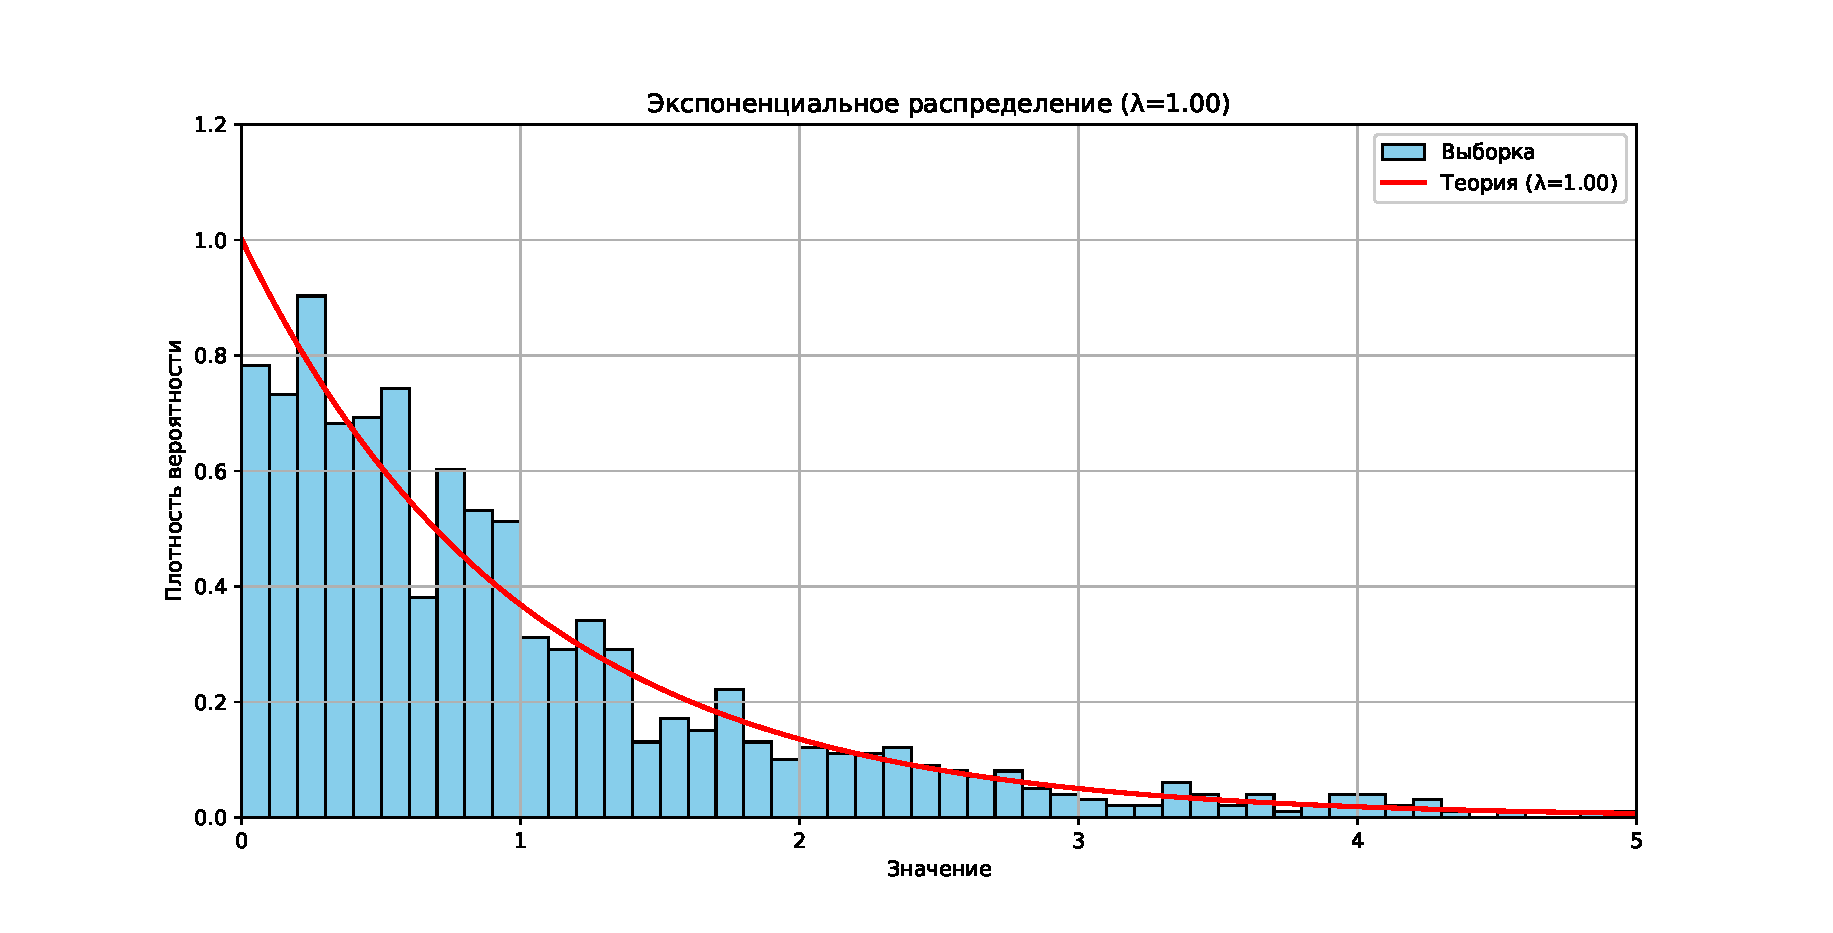
\includegraphics[width=1\textwidth]{data/ex3/exp.eps}
\caption{Результат моделирования экспоненциального распределения (размер выборки N = 1000, \(\lambda = 1.\))}
\end{figure}
\begin{figure}[H]
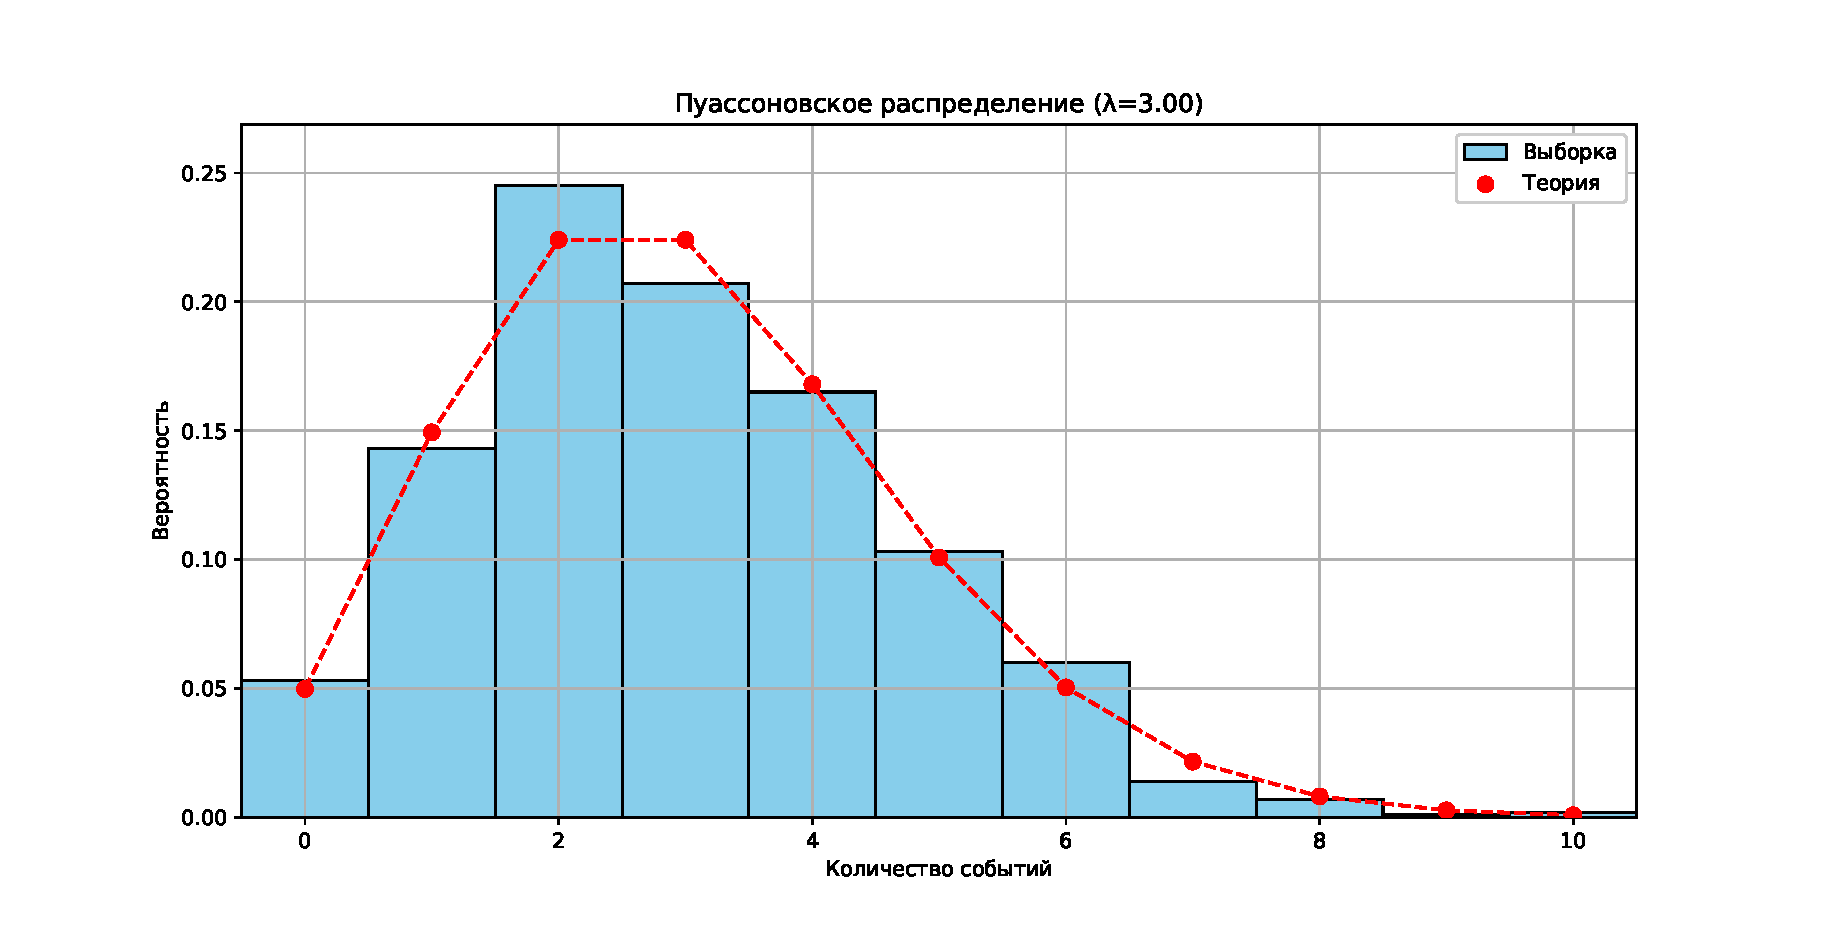
\includegraphics[width=1\textwidth]{data/ex3/pois_exp.eps}
\caption{Результат моделирования пуассоновского распределения через экспоненциальное (размер выборки N = 1000, \(\lambda = 3.\))}
\end{figure}
\begin{figure}[H]
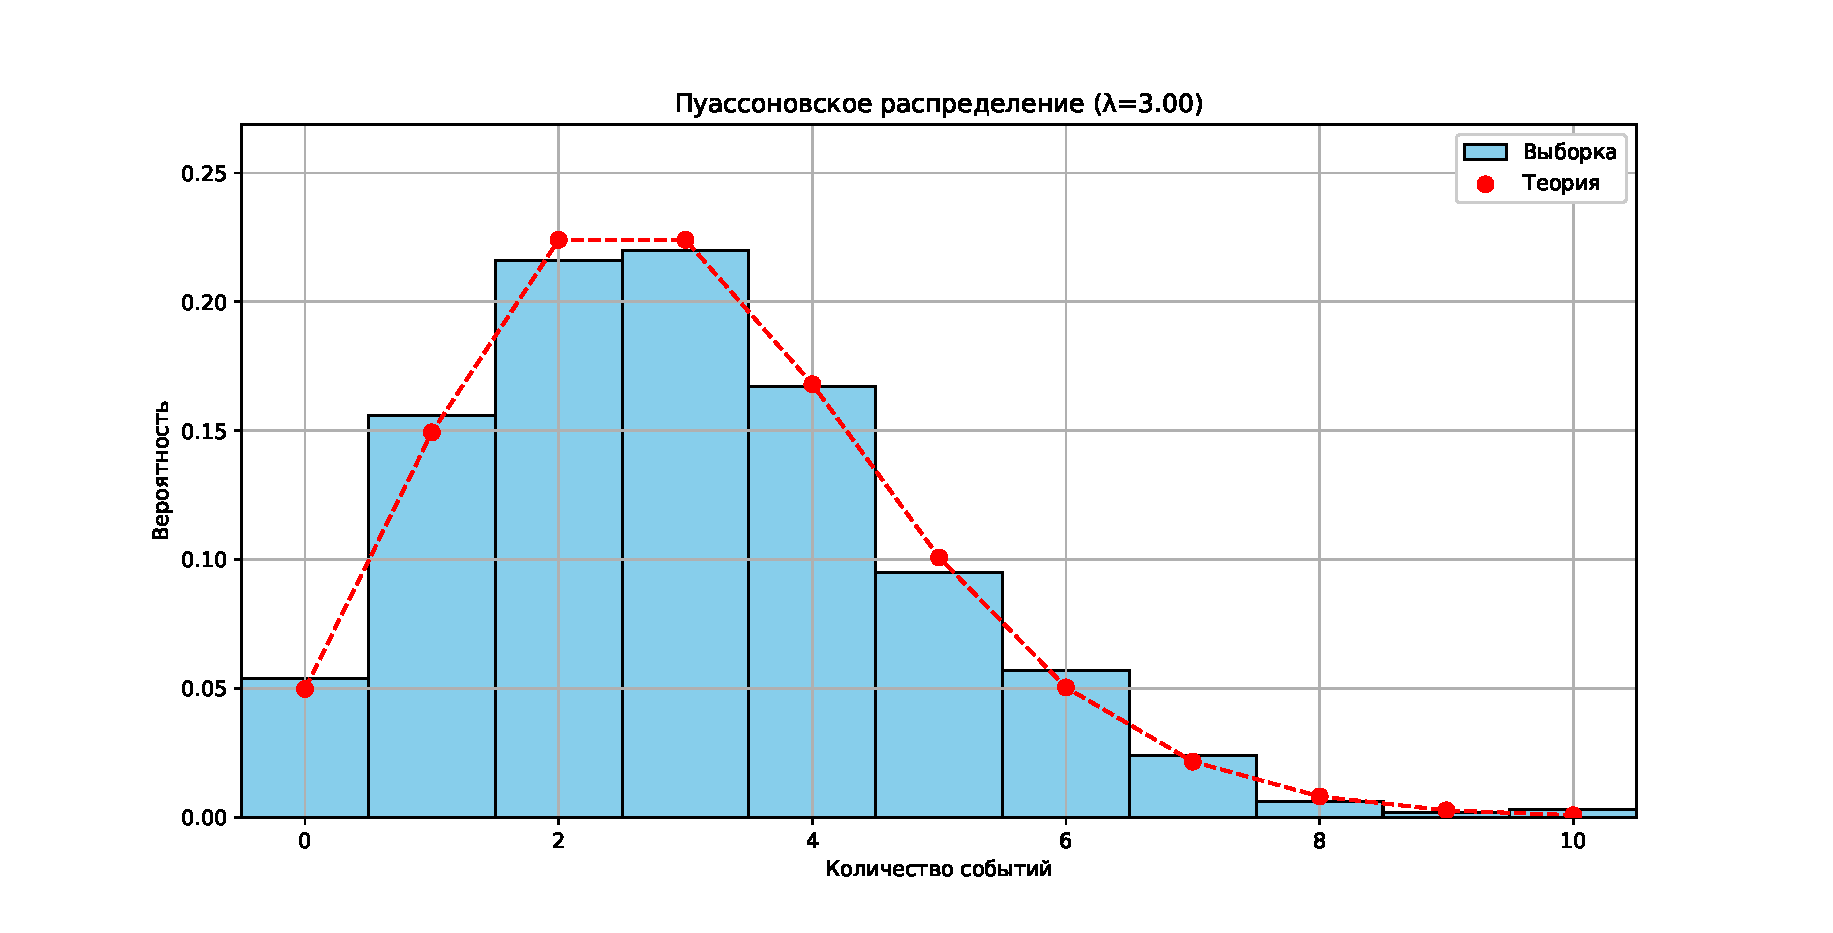
\includegraphics[width=1\textwidth]{data/ex3/pois_bin.eps}
\caption{Результат моделирования пуассоновского распределения через биномиальное (размер выборки N = 1000, \(\lambda = 3.\))}
\end{figure}
Используем критерий согласия Пирсона. По результатам работы программы значение функции распределения \(\chi^2_{k-1}\) на статистике \(\chi^2\) меньше уровня значимости в 54 случаях из 1000. Таким образом, в 94.6\% случаев гипотеза о порождении выборки пуассоновским распределением принимается.
\begin{figure}[H]
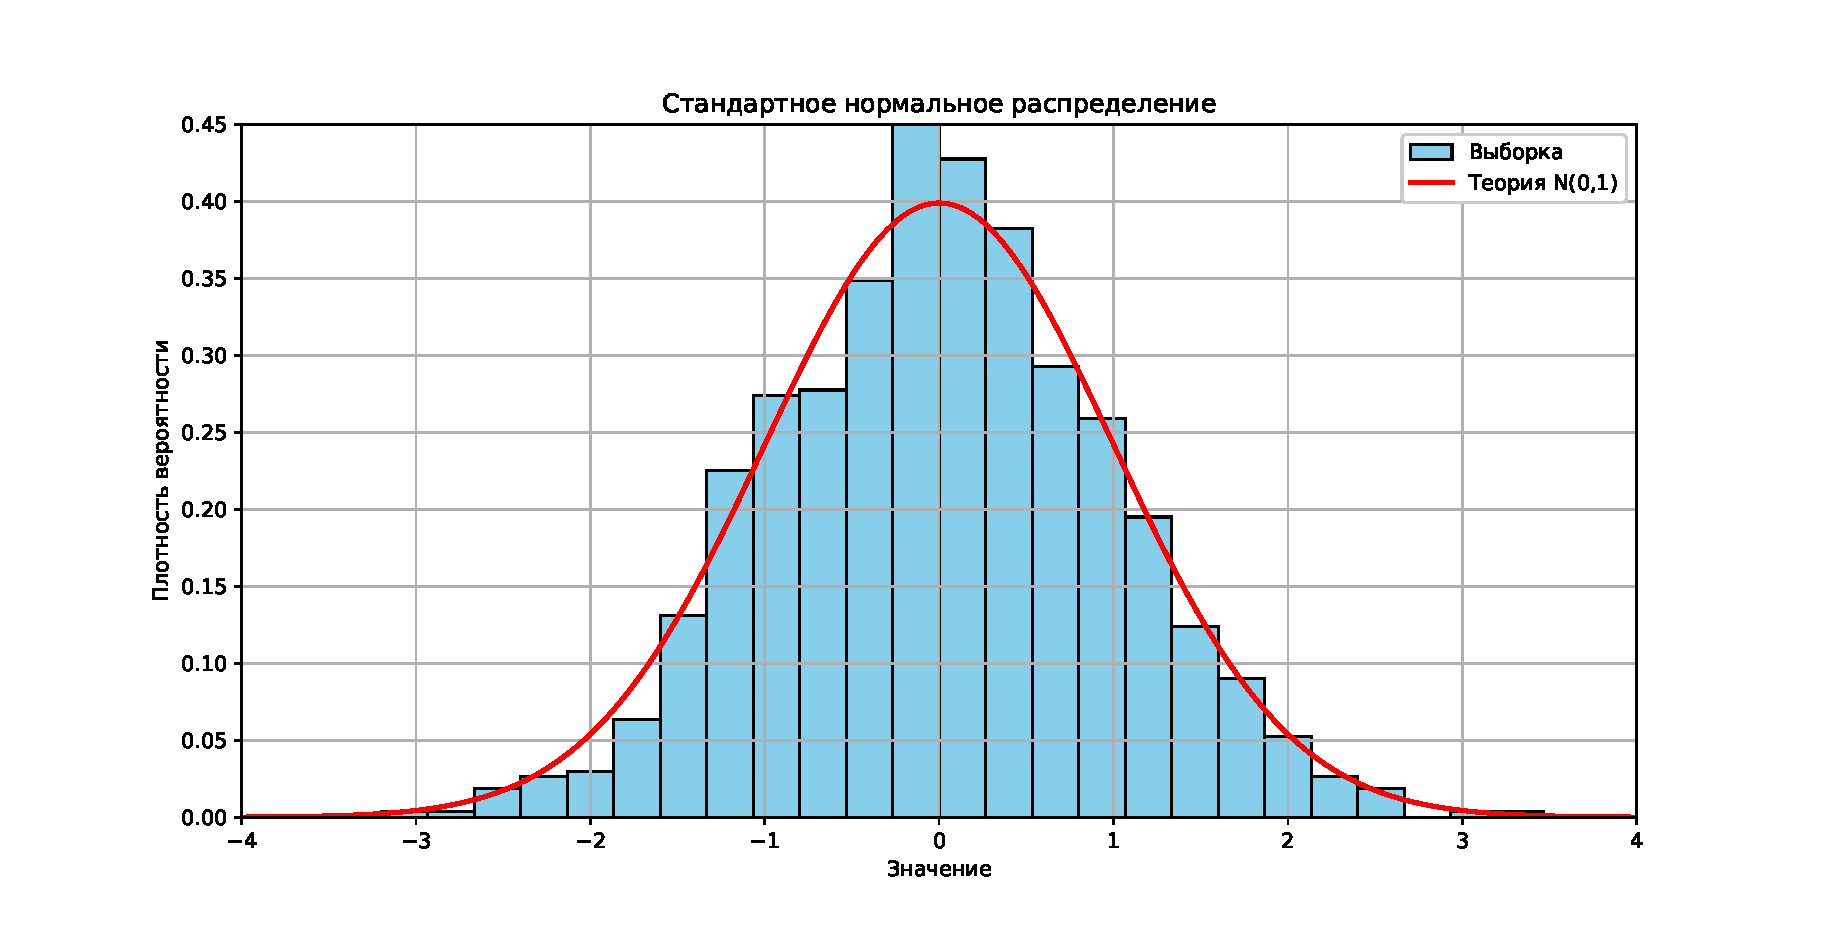
\includegraphics[width=1\textwidth]{data/ex3/stand_norm.eps}
\caption{Результат моделирования стандартного нормального распределения (размер выборки N = 1000.}
\end{figure}
Применим критерий Стьюдента. Получаем, что гипотеза о нормальной распределенности выборки принимается в 93.8\% случаев.
Аналогично, применяя критерий Фишера, получаем, что гипотеза принимается в 94.9\% случаев.

Заметим, что процент случаев, когда гипотеза отклоняется, в среднем соответствует выбранному уровню значимости \(\alpha = 0.05\).

\section{Задание 4}
\subsection{Постановка задачи}
\begin{enumerate}
    \item Построить датчик распределения Коши.
\item На основе датчика распределения Коши с помощью метода фон Неймана построить датчик стандартного нормального распределения. При помощи графика normal probability plot убедиться в корректности построенного датчика и
обосновать наблюдаемую линейную зависимость.
\item Сравнить скорость моделирования стандартного нормального распределения в
задании 3 и в задании 4.
\end{enumerate}

\subsection{Теоретические сведения}

\subsubsection{Датчик распределения Коши}

Распределение Коши $C(x_0, \gamma)$ с параметрами $x_0 \in \mathbb R$ и $\gamma > 0$ имеет следующую функцию распределения:
$$
    F_X(x) = \frac{1}{\pi}\arctan(\frac{x - x_0}{\gamma}) + \frac{1}{2}
$$
Воспользуемся тем, что если $U \sim \mathcal U[0, 1]$, то $X = x_0 + \gamma\tan\left(\pi\left(U - \frac{1}{2}\right)\right) \sim C(x_0, \gamma)$

\subsubsection{Rejection sampling}

Метод Фон Неймана, или же rejection sampling, это метод генерации выборки некоторого распределения. Будем генерировать выборку из стандартного нормального распределения при помощи распределения Коши. Для этого понадобятся их плотности. Плотность стандартного нормального распределения:
$$
    f(x) = \frac{1}{\sqrt{2\pi}}e^{-\frac{x^2}{2}}.
$$
Плотность стандартного распределения Коши ($x_0 = 0, \gamma = 1$):
$$
    g(x) = \frac{1}{\pi} \frac{1}{x^2 + 1}.
$$

\begin{figure}[H]
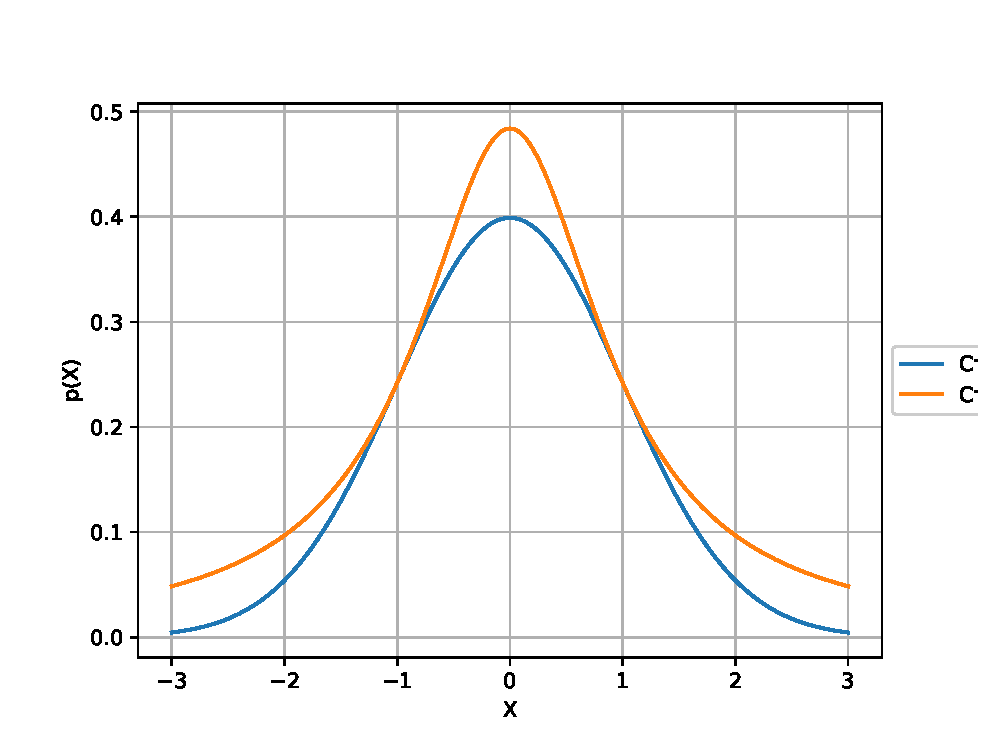
\includegraphics[width=1\textwidth]{data/ex4/cauchy_norm.eps}
\caption{сравнение плотностей стандартного нормального распределения и стандартного распределения Коши.}
\end{figure}

Для метода Фон Неймана понадобится найти константу $M$, для которой выполнено: $\frac{f(x)}{Mg(x)} \le 1\ \forall x \in \mathbb R$. Будем искать супремум отношения $r(x) = \frac{f(x)}{g(x)}$ (Чем меньше константа, тем быстрее работает метод, так что оптимальнее всего выбрать минимальное значение):
$$r(x) = \frac{f(x)}{g(x)} = \sqrt\frac{\pi}{2}(x^2 + 1)e^{-\frac{x^2}{2}}$$
$$r'(x) = \sqrt\frac{\pi}{2}\left(xe^{\frac{-x^2}{2}} - (x^2 + 1)\frac{x^2}{2}xe^{-\frac{x^2}{2}}\right) = \sqrt\frac{\pi}{2}xe^{-\frac{x^2}{2}}\frac{1}{2}\left(2 - x^4 - x^2\right) = 0 \Rightarrow x = 0,\, x = \pm 1.$$
$$r(0) = \sqrt\frac{\pi}{2},\, r(\pm 1) = \sqrt\frac{2\pi}{e}. \sqrt\frac{2\pi}{e} > \sqrt\frac{\pi}{2} \Rightarrow M = \sqrt\frac{2\pi}{e}.$$

Смысл метода в том, что мы генерируем значение из известного распределения $x$ и принимаем его в выборку целевого распределения с вероятностью $\frac{f(x)}{Mg(x)}$. Обоснуем применимость метода. Рассмотрим плотность вероятности при условии, что мы приняли значение:
$$
    p(x|A) = \frac{\mathbb{P}(A|x)p(x)}{\mathbb{P}(A)} = \frac{\frac{f(x)}{Mg(x)}g(x)}{\mathbb{P}(A)}
$$
$$
    \mathbb P(A) = \int_{-\infty}^{+\infty} \frac{f(x)}{Mg(x)} g(x) \mathrm dx = \int_{-\infty}^{+\infty} \frac{f(x)}{M} \mathrm dx = \frac{1}{M}
$$
$$
    p(x|A) = \frac{\frac{f(x)}{Mg(x)}g(x)}{\frac{1}{M}} = f(x)
$$
Таким образом, мы получаем нужную плотность распределения.

Далее будем проверять корректность при помощи метода normal probability plot. Для этого отсортируем выборку и выведем ее на плоскость, где в качестве координаты y будем использовать теоретические квантили нормального распределения.

Любое нестандартное нормальное распределение можно представить в виде $\mu + \sigma \mathcal N(0, 1)$, то есть в виде линейного преобразования стандартного, поэтому график также будет линейным. Для других распределений квантили ведут себя по другому, поэтому график не будет линейным. Также графики не будут инвариантны относительно параметров масштаба и сдвига.

\subsection{Результаты работы программы}
\begin{figure}[H]
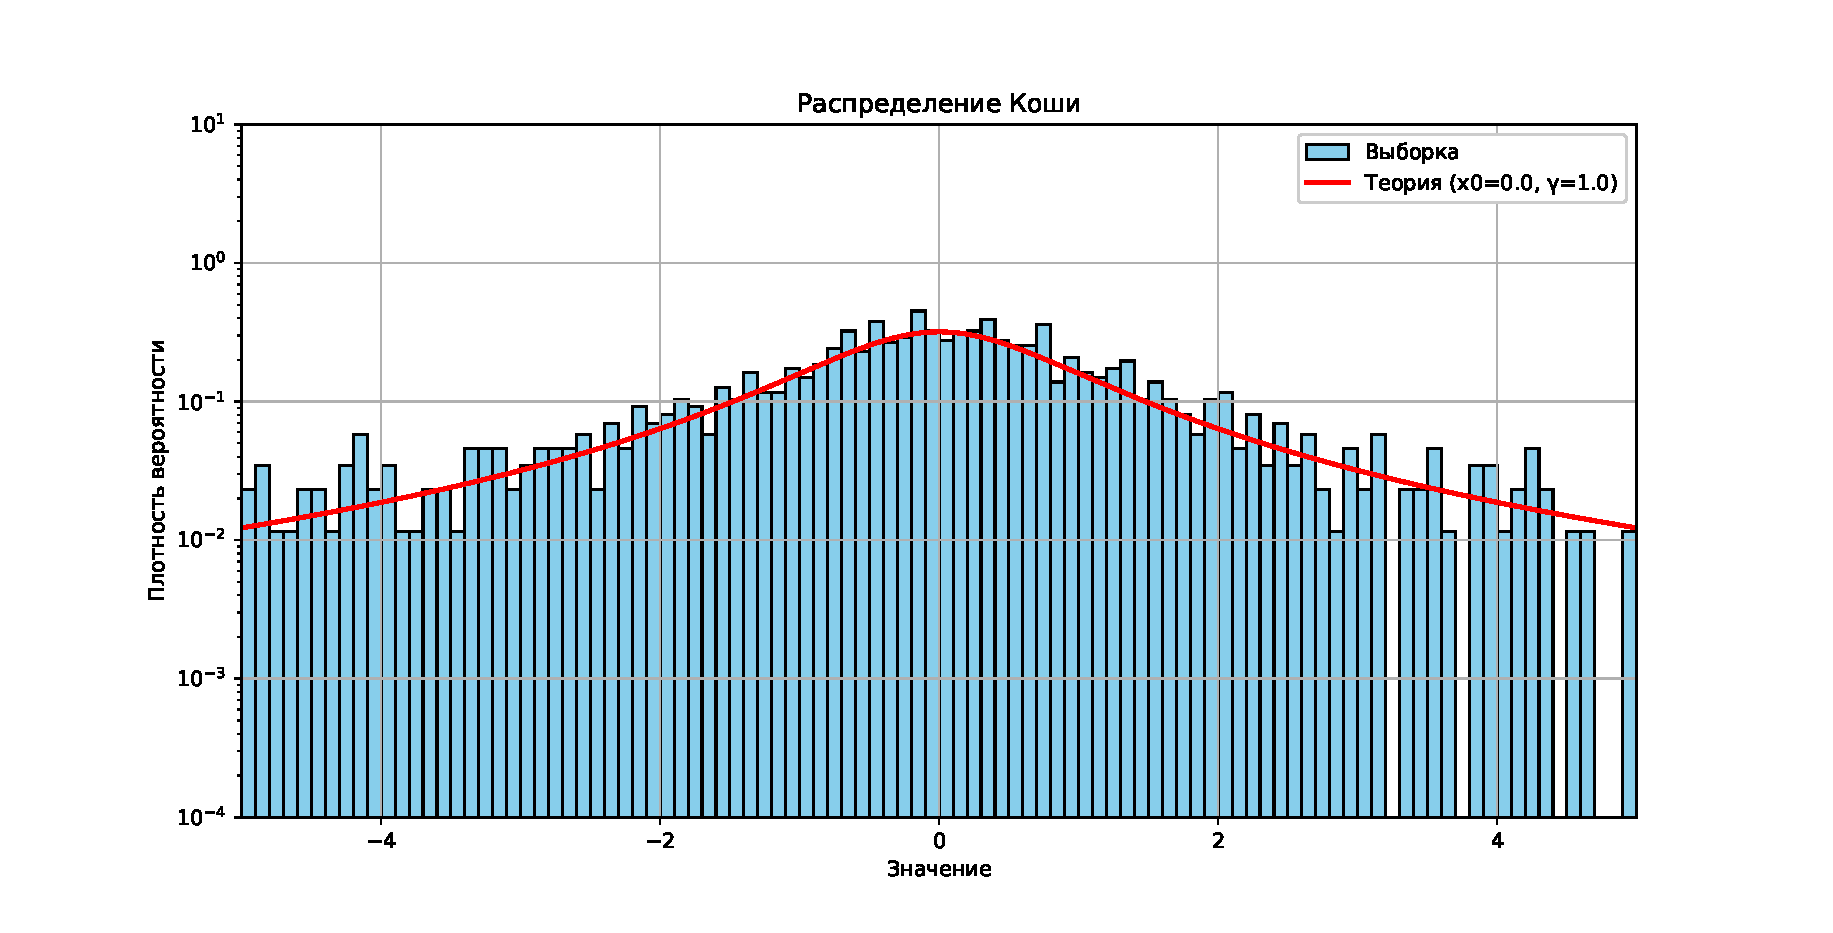
\includegraphics[width=1\textwidth]{data/ex4/cauchy.eps}
\caption{Результат моделирования распределения Коши (размер выборки N = 1000, \(x_0 = 1,\, \gamma = 1\)).}
\end{figure}

\subsection{Результаты работы программы}
\begin{figure}[H]
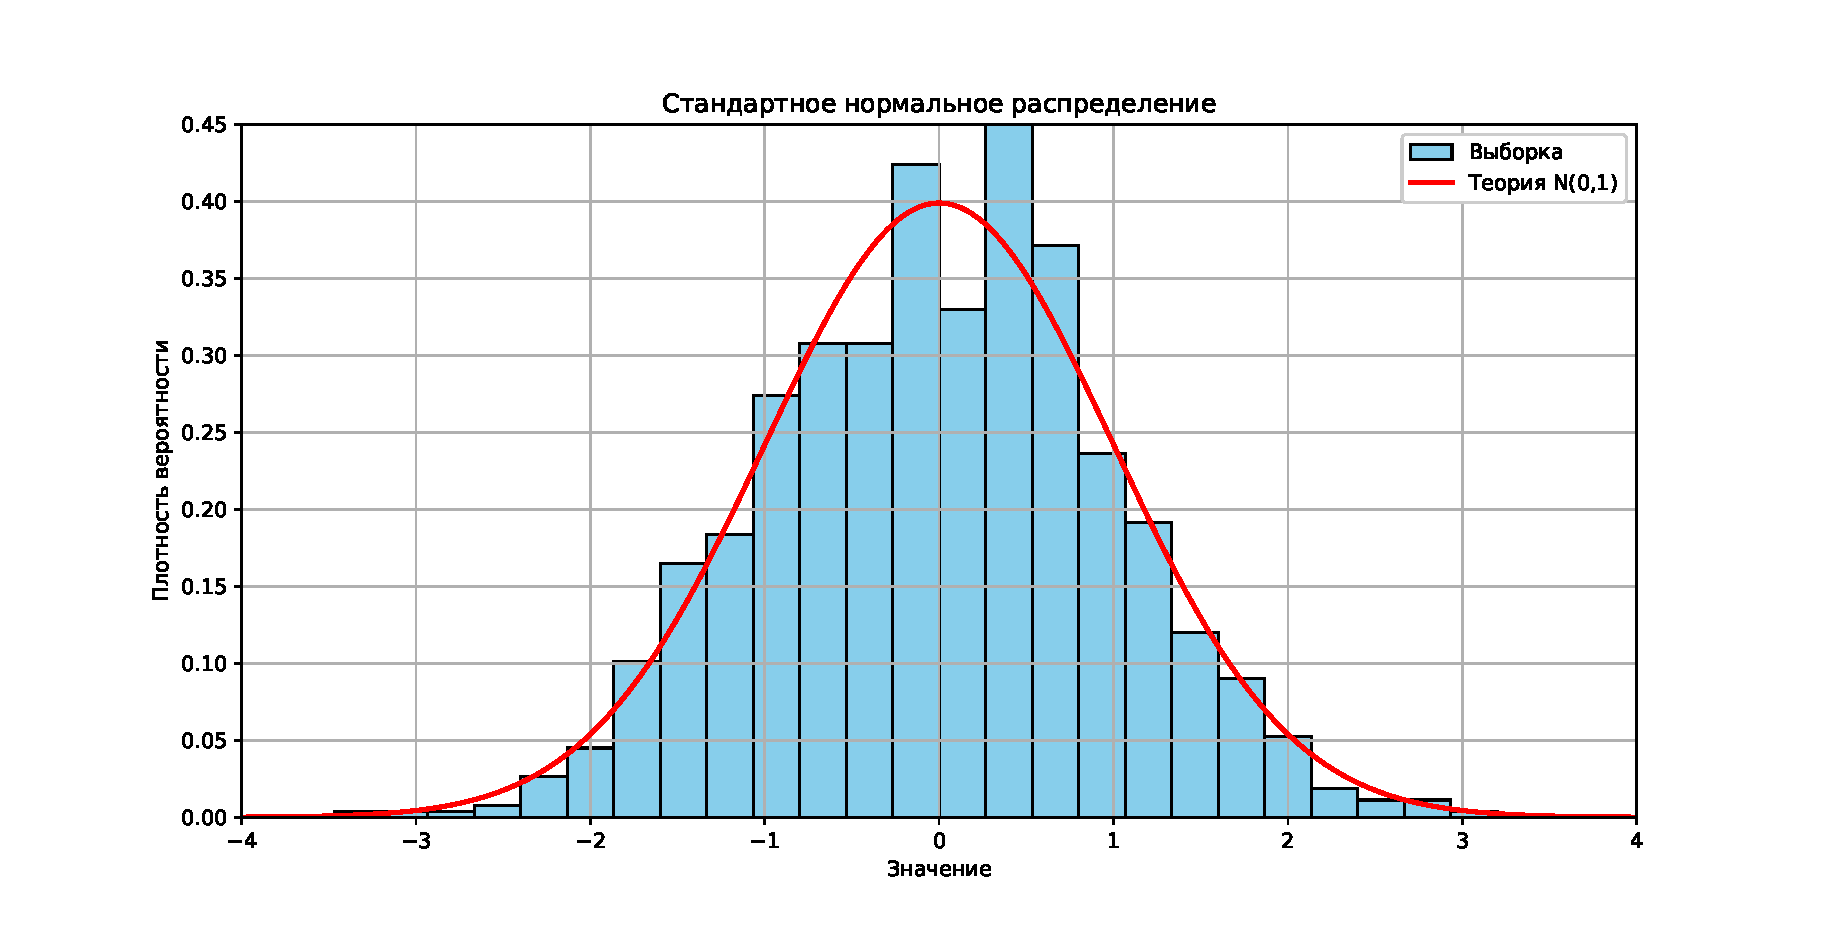
\includegraphics[width=1\textwidth]{data/ex4/norm.eps}
\caption{Результат моделирования стандартного нормального распределения методом random sampling (размер выборки N = 1000).}
\end{figure}

\subsection{Результаты работы программы}
\begin{figure}[H]
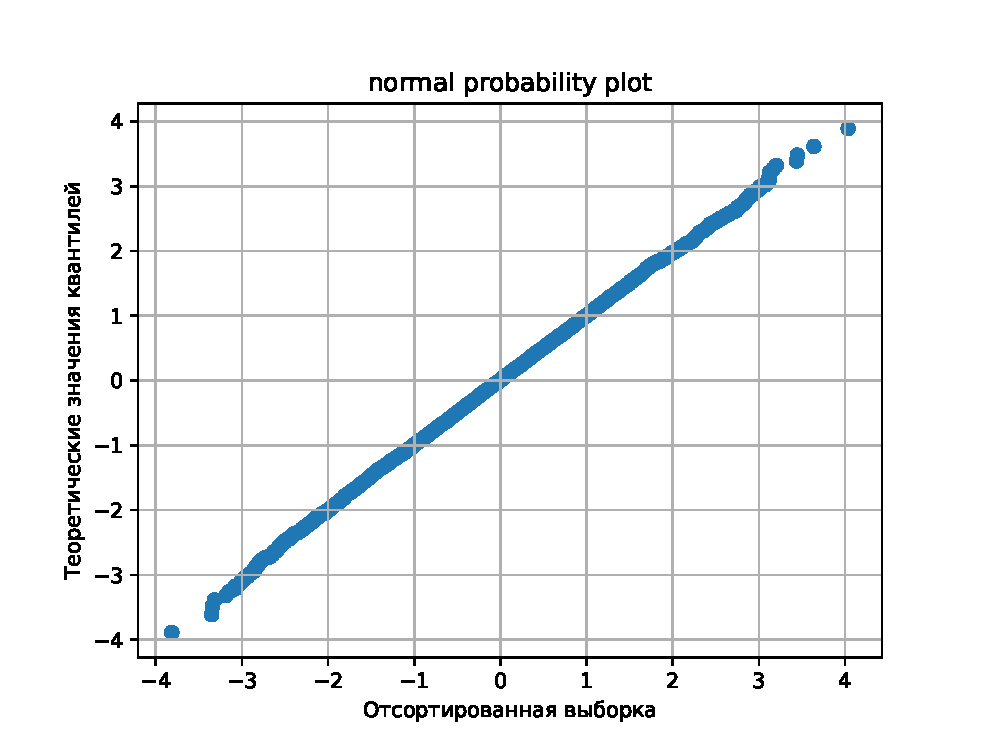
\includegraphics[width=1\textwidth]{data/ex4/npp.eps}
\caption{Normal probability plot для получившейся выборки (размер выборки N = 10000).}
\end{figure}
Видно, что график является очень близким к линейному, поэтому гипотезу о нормальной распределенности выборки следует принять.

Сравним скорости работы методов Бокса-Мюллера и random sampling на разных размерах выборки:
\subsection{Результаты работы программы}
\begin{figure}[H]
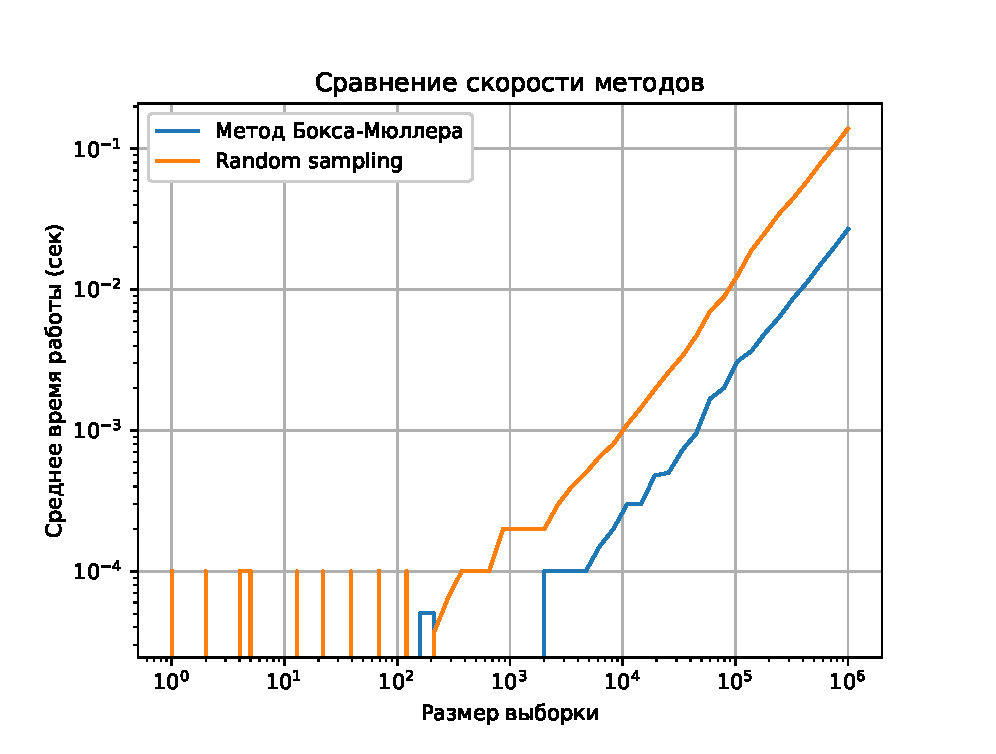
\includegraphics[width=1\textwidth]{data/ex4/comp.eps}
\end{figure}

Видно, что метод Бокса-Мюллера на порядок быстрее, чем random sampling.


\section{Задание 5}
\subsection{Постановка задачи}
\begin{enumerate}
    \item Пусть \(X_i \sim \mathcal{N}(\mu,\sigma^2)\). Убедиться эмпирически в справедливости теоремы о законе больших чисел (ЗБЧ) и центральной предельной теоремы (ЦПТ): исследовать поведение суммы \(S_n = \sum_{i = 1}^nX_i\) и эмпирического распределения величины \(\sqrt{n}\frac{S_n}{n} - a\).
\item Считая \(\mu,\,\sigma\) неизвестными, построить доверительные интервалы для среднего и
дисперсии по имеющейся выборке.
\item Пусть \(X_i \sim K(a, b)\) — имеет распределение Коши с параметром сдвига \(a\) и масштаба \(b\). Изучить эмпирически как ведут себя суммы \(\frac{S_n}{n}\), объяснить результат и найти закон распределения данных сумм.
\end{enumerate}

\subsection{Теоретические сведения}

\subsubsection{ЗБЧ и ЦПТ}
Рассмотрим независимые одинакого распределенные случайные величины: $X_i \sim \mathcal{N} (\mu, \sigma^2)$. Убедимся эмприрически в справедливости закона больших чисел (ЗБЧ) и центральной предельной теоремы (ЦПТ). Рассмотрим среднее $M_n = \frac{X_1 + \dots + X_n}{n}$. ЗБЧ гласит, что $M_n \xrightarrow[n \to \infty]{p} \mu$.

ЦПТ гласит, что $Y = \frac{S_n - \mu n}{\sigma \sqrt n} \xrightarrow[n \to \infty]{d} \mathcal{N}(0, 1)$, где $S_n = X_1 + \dots + X_n$. Сходимость по распределению означает, что распределение получившейся величины близко к целевому.

\subsubsection{Доверительные интервалы}

Доверительным интервалом называется интервал, которому принадлежит неизвестный параметр с заданной вероятностью. Для нормального распределения рассмотрим симметричный доверительный интервал, то есть $\mathbb P(-\gamma < S < \gamma) = \alpha$. в данном случае требуется найти доверительный интервал для матожидания и дисперсии по выборке из нормального распределения $X_1, \dots, X_n$.

В случае матожидания рассмотрим случайную величину
$$
    T = \sqrt n \frac{M - \mu}{s},
$$
где $M = \frac{X_1 + \dots + X_n}{n}$ --- выборочное среднее, $s = \sqrt{\frac{\sum_{i = 1}^n(X_i - M)^2}{n-1}}$ --- несмещенное выборочное стандартное отклонение. Известно, что эта величина имеет распределение Стьюдента с $n - 1$ степенями свободы. Пусть $t_{\alpha, n-1}$ --- $\alpha$-квантиль распределения Стьюдента. Тогда в силу симметрии квантилей имеем:
$$
    \mathbb{P}(-t_{1-\frac{1-\alpha}{2},n-1} < T < t_{1-\frac{1-\alpha}{2},n-1}) = \alpha
$$
$$
    \mathbb{P}(-t_{1-\frac{1-\alpha}{2},n-1} < \sqrt n \frac{M - \mu}{s} < t_{1-\frac{1-\alpha}{2},n-1}) = \alpha
$$
$$
    \mathbb{P}(-t_{1-\frac{1-\alpha}{2},n-1}\frac{s}{\sqrt n} + M < \mu < t_{1-\frac{1-\alpha}{2},n-1}\frac{s}{\sqrt n} + M) = \alpha
$$
Таким образом, доверительный интервал имеет вид
$$
    [-t_{1-\frac{1-\alpha}{2},n-1}\frac{s}{\sqrt n} + M, t_{1-\frac{1-\alpha}{2},n-1}\frac{s}{\sqrt n} + M].
$$

В случае дисперсии рассмотрим случайную величину
$$
    H = \frac{(n - 1)s^2}{\sigma^2}.
$$
Известно, что она имеет распределение $\chi^2(n - 1)$. Имеем:
$$
    \mathbb{P}(\chi^2_{\frac{1-\alpha}{2},n-1} < H < \chi^2_{1-\frac{1-\alpha}{2},n-1}) = \alpha
$$
$$
    \mathbb{P}(\chi^2_{\frac{1-\alpha}{2},n-1} < \frac{(n - 1)s^2}{\sigma^2} < \chi^2_{1-\frac{1-\alpha}{2},n-1}) = \alpha
$$
$$
    \mathbb{P}(\frac{(n-1)s^2}{\chi^2_{1-\frac{1-\alpha}{2},n-1}} < \sigma^2 < \frac{(n-1)s^2}{\chi^2_{\frac{1-\alpha}{2},n-1}}) = \alpha
$$
Следовательно, доверительный интервал имеет вид
$$
    [\frac{(n-1)s^2}{\chi^2_{1-\frac{1-\alpha}{2},n-1}}, \frac{(n-1)s^2}{\chi^2_{\frac{1-\alpha}{2},n-1}}].
$$

\subsubsection{Средние распределения Коши}

Пусть $X_i \sim K(a, b)$ --- распределение Коши с параметром сдвига a и масштаба b. Изучим, как ведут себя средние $M_n = \frac{S_n}{n} = \frac{X_1 + \dots + X_n}{n}$. Посмотрим на их распределение при некотором большом $n$:

\begin{figure}[H]
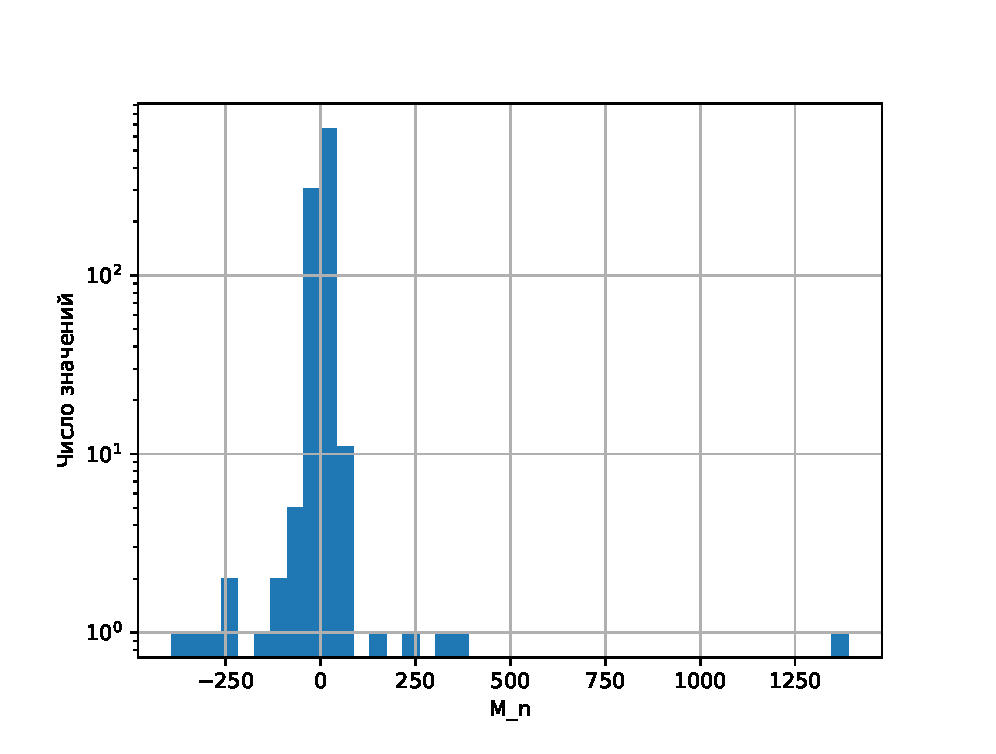
\includegraphics[width=1\textwidth]{data/ex5/Cauchy_M.eps}
\end{figure}

Видим, что присутствуют сильные выбросы, то есть величина не сходится. Это вызвано тем, что у распределения Коши тяжелые хвосты. Покажем, что среднее имеет распределение Коши с теми же параметрами. Рассмотрим характеристическую функцию распределения Коши:
$$
    \varphi_X(x) = \mathbb E(e^{itX}) = e^{ita + b|t|}
$$
Тогда в силу независимости
$$
    \varphi_{M_n}(x) = \prod_{k = 1}^n \mathbb E(e^{it\frac{X_k}{n}}) = \left(e^{\frac{ita + b|t|}{n}}\right)^n = e^{ita + b|t|}
$$
Таким образом, среднее имеет то же распределение, что и слагаемые.

\subsection{Результаты работы программы}

\subsubsection{ЗБЧ и ЦПТ}

\begin{figure}[H]
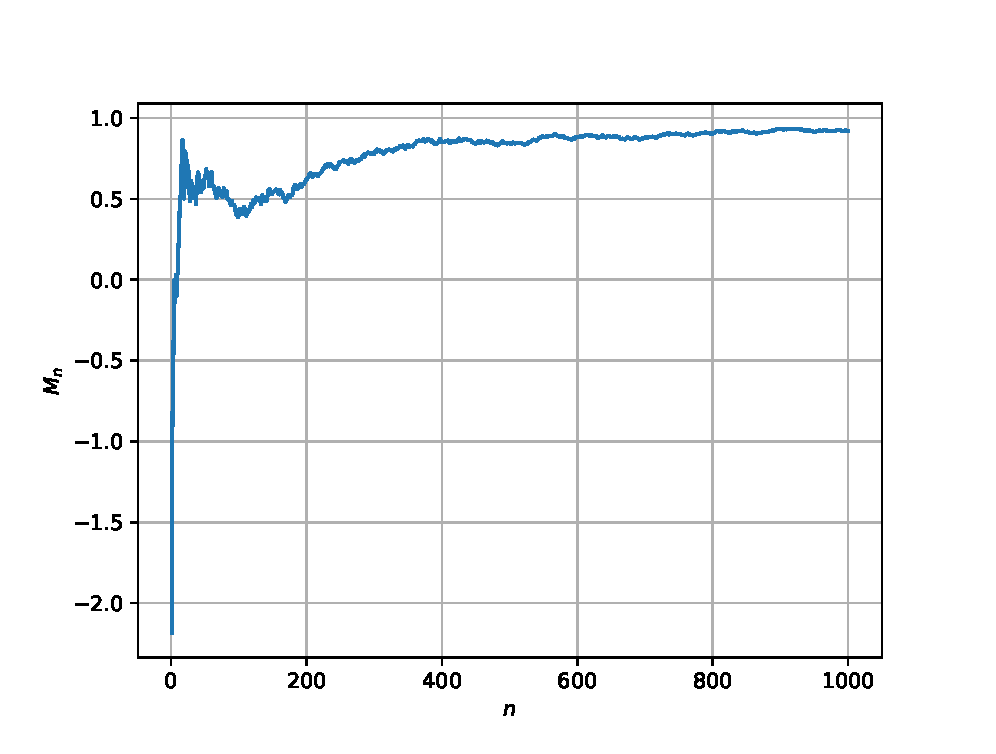
\includegraphics[width=1\textwidth]{data/ex5/zbch.eps}
\caption{Визуализация ЗБЧ для \(\mathcal{N}(1, 2)\) (средние \(M_n \to \mu = 1\))}
\end{figure}

\begin{figure}[H]
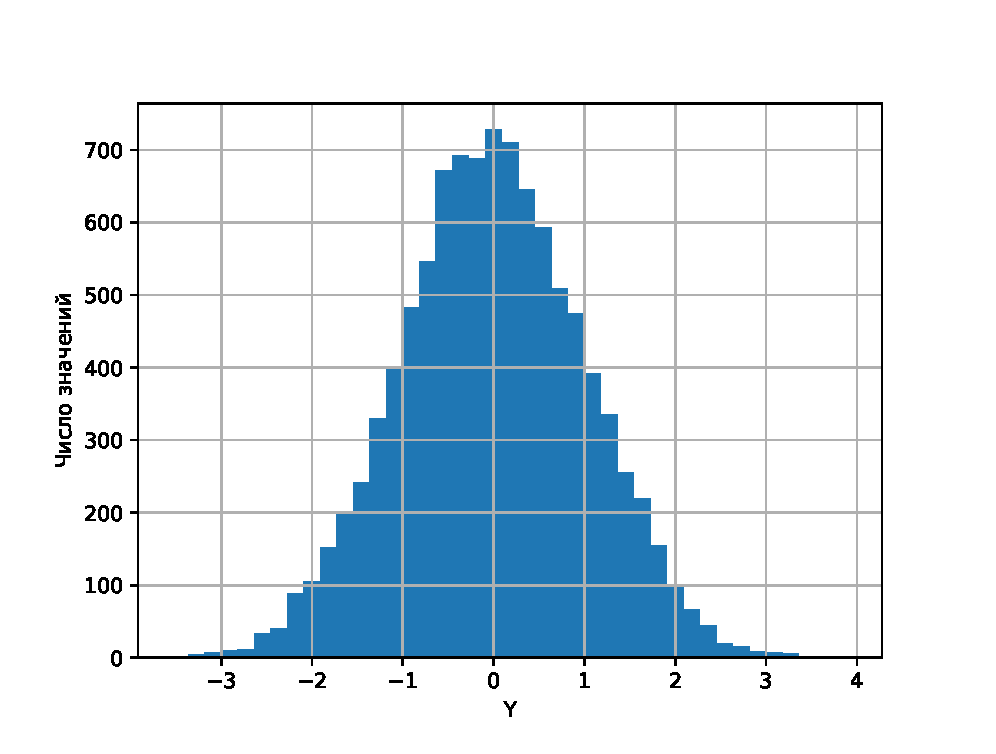
\includegraphics[width=1\textwidth]{data/ex5/cpt.eps}
\caption{Визуализация ЦПТ для \(\mathcal{N}(1, 2)\) ($Y = \frac{S_n - \mu n}{\sigma \sqrt n} \xrightarrow[n \to \infty]{d} \mathcal{N}(0, 1)$). Видно, что распределение соответствует стандартному нормальному.}
\end{figure}

\subsubsection{Доверительные интервалы}

Покажем эволюцию интервалов при росте объема выборки для \(\mathcal{N}(2, 0.5)\):

\begin{figure}[H]
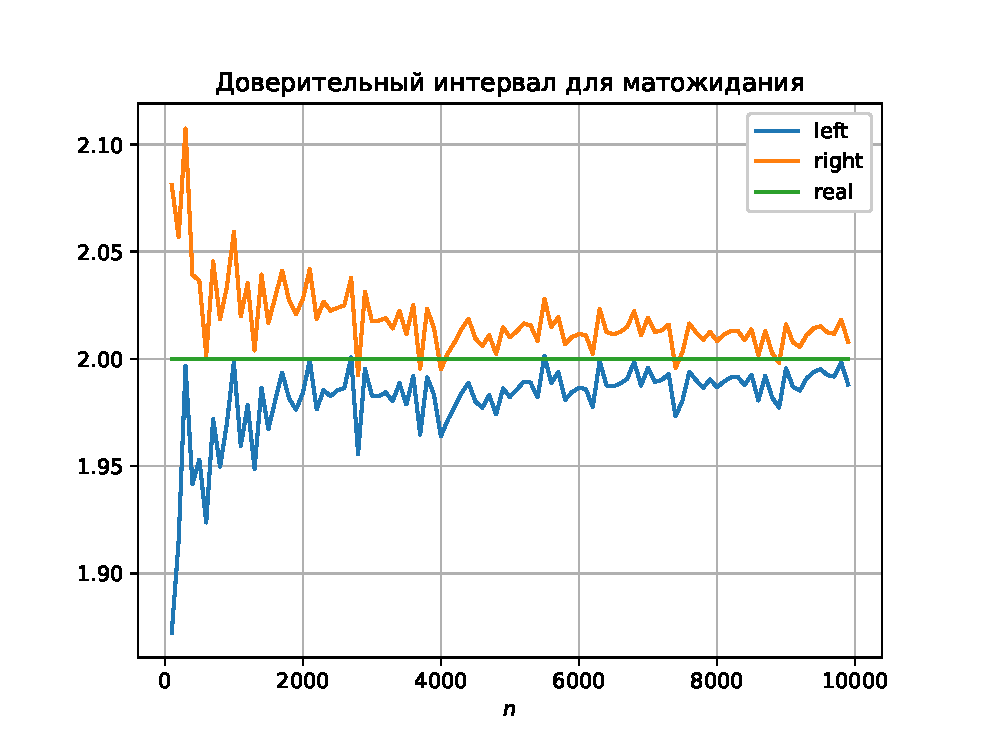
\includegraphics[width=1\textwidth]{data/ex5/MO_CI.eps}
\end{figure}
\begin{figure}[H]
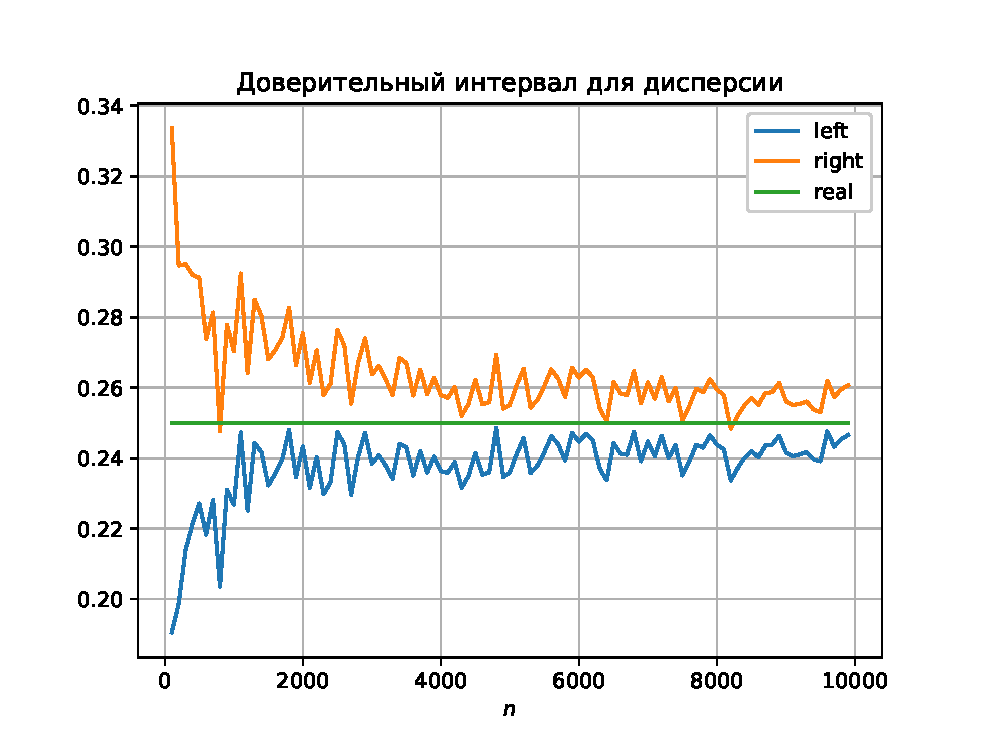
\includegraphics[width=1\textwidth]{data/ex5/disp_CI.eps}
\end{figure}



\section{Задание 6}
\subsection{Постановка задачи}
\begin{enumerate}
    \item Вычислить следующий интеграл:
    $$
    I = \int_{-\infty}^{+\infty} \int_{-\infty}^{+\infty} \dots \int_{-\infty}^{+\infty} \frac{e^{-\left(x_1^2 + \dots + x_{10}^2 + \frac{1}{2^7\cdot x_1^2 \cdot \dots \cdot x_{10}^2}\right)}}{x_1^2 \cdot \dots \cdot x_{10}^2} \mathrm{d}x_1 \mathrm{d} x_2 \dots \mathrm{d} x_{10}
    $$
        \begin{enumerate}
            \item Методом Монте-Карло
            \item Методом квадратур, сводя задачу к вычислению собственного интеграла Римана.
        \end{enumerate}
    \item Оценить точность вычислений для каждого из двух случаев.
\end{enumerate}

\subsection{Теоретические сведения}

\subsubsection{Метод Монте Карло}

Метод Монте Карло заключается в том, что некий случайный процесс многократно моделируется, а потом на его основе высчитываются нужные характеристики. В случае интегрирования стандартный метод заключается в следующем:

Пусть нужно вычислить интеграл

$$
    \int_a^b f(x) \mathrm{d}x
$$
Рассмотрим случайную величину $u$, равномерно распределенную на отрезке $[a, b]$. Тогда $f(u)$ --- тоже случайная величина, причем
$$
    \mathbb{E}f(u) = \int_a^b f(x) \varphi(x) \mathrm{d}x,
$$
где $\varphi(x) = \frac{1}{b-a}$ --- плотность случайной величины $u$. Таким образом,
$$
    \int_a^b f(x) \mathrm{d}x = (b - a) \mathbb{E}f(u),
$$
но матожидание $f(u)$ можно легко оценить, смоделировав эту случайную величину и посчитав выборочное среднее.

Применим похожую идею для данной задачи. Пусть случайные величины $X_i,\, i = \overline{1, 10}$ имеют нормальное распределение. Их плотность распределения имеет вид
$$
    p_i(x_i) = \frac{1}{\sqrt{2\pi}\sigma}e^{-\frac{1}{2}\left(\frac{x_i - \mu}{\sigma}\right)^2},
$$
где $\mu$ --- матожидание, $\sigma^2$ --- дисперсия. Взяв $\mu = 0$ и $\sigma = \frac{1}{\sqrt 2}$, имеем
$$
    p_i(x_i) = \frac{1}{\sqrt \pi}e^{-x_i^2}.
$$
Тогда вектор $X = (X_1, \dots, X_{10})$ имеет имеет плотность распределения
$$
    p(x) = \prod_{i = 1}^{10} p_i(x_i) = \frac{1}{\pi^5}e^{-(x_1^2 + \dots + x_{10}^2)},
$$
где $x = (x_1, \dots, x_{10})$. Пусть $y = \frac{1}{x_1^2 \cdot \dots \cdot x_{10}^2},\,f(x) = \pi^5 ye^{-\frac{y}{2^7}}$, тогда
$$
    I = \int_{\mathbb{R}^{10}} f(x)p(x)\mathrm{d}x = \mathbb{E}f(X).
$$
Таким образом, достаточно промоделировать нормальный вектор $X$ достаточное число раз, посчитать $f(X)$ и найти среднее $\overline X_n = \frac{1}{n}\sum_{k = 1}^n f(X_k)$ как приближение матожидания.

Оценим ошибку через неравенство Чебышёва:
$$
    \mathbb{P}(|\overline X_n - \mathbb E X| \ge \varepsilon) \le \frac{\mathbb{D} X}{n \varepsilon^2}.
$$
Для оценки дисперсии используем несмещенную выборочную дисперсию:
$$
    s^2_n = \frac{1}{n-1}\sum_{k = 1}^n (X_k - \overline X)^2.
$$
При достаточно больших $n\ (n \ge 100)$ эта оценка будет иметь высокую точность.
Таким образом,
$$
    \mathbb{P}(|\overline X_n - \mathbb E X| \ge \varepsilon) \le \frac{s^2_n}{n \varepsilon^2} = 1 - \alpha.
$$

\subsubsection{Метод квадратур}

Воспользуемся методом прямоугольников. Для этого сделаем замену
$$
    x_i = \tan(x_i),\, \mathrm dx_i = \frac{\mathrm dy_i}{\cos^2y_i},\, i = \overline{1, 10}.
$$
Интеграл принимает вид
$$
    \int_{-\frac{\pi}{2}}^{\frac{\pi}{2}} \dots \int_{-\frac{\pi}{2}}^{\frac{\pi}{2}} \exp\left(-\sum_{i = 1}^{10} \tan^2 y_i - 2^{-7}\prod_{i = 1}^{10}\cot^2 y_i\right)\prod_{i = 1}^{10}\cot^2 y_i\prod_{i = 1}^{10}\frac{1}{\cos^2 y_i} \mathrm dy_1 \dots \mathrm dy_{10} =
$$
$$
     = \int_{-\frac{\pi}{2}}^{\frac{\pi}{2}} \dots \int_{-\frac{\pi}{2}}^{\frac{\pi}{2}} \exp\left(-\sum_{i = 1}^{10} \tan^2 y_i - 2^{-7}\prod_{i = 1}^{10}\cot^2 y_i\right)\prod_{i = 1}^{10}\frac{1}{\sin^2 y_i} \mathrm dy_1 \dots \mathrm dy_{10} =
$$
$$
    = \int_{[-\frac{\pi}{2}, \frac{\pi}{2}]^{10}}f(y)dy = 2^{10}\int_{[0, \frac{\pi}{2}]^{10}}f(y)dy,
$$
где
$$
    y = (y_1, \dots, y_{10}),\, f(y) = \exp\left(-\sum_{i = 1}^{10} \tan^2 y_i - 2^{-7}\prod_{i = 1}^{10}\cot^2 y_i\right)\prod_{i = 1}^{10}\frac{1}{\sin^2 y_i}.
$$
Будем пользоваться методом следних прямоугольников. Для вычисления интеграла составим разбиение отрезка $[0, \frac{\pi}{2}]$ на N частей и получим серединные точки: $T = \{\frac{h}{2}, \frac{h}{2} + h, \dots, \frac{h}{2} + (N-1)h\} = \{T_0, \dots, T_{N-1}\}$, где $h = \frac{\pi}{2 N}$. Возведем в 10 декартову степень для получения 10--мерной сетки. Итоговая формула для численного вычисления интеграла:
$$
    I = 2^{10}\sum_{x \in T^{10}}f(x)h^{10}.
$$

Можно существенно сократить вычисления, заметив, что функция не меняет значение при перестановке аргументов. Тогда интеграл можно записать как
$$
    I = \sum_{0 \le k_1 \le k_2 \le \dots \le k_{10} \le N-1} \frac{N!}{n_1!\cdot \dots \cdot n_{N}!} f(T_{k_1}, \dots, T_{k_{10}}),
$$
где $n_i, i = \overline{1, N}$ --- число индексов, равных $i - 1$.

Оценим погрешность. Разложим $f(\mathbf{x})$ в ряд Тейлора вокруг центра $\mathbf{c}$ гиперкуба:
$$
f(\mathbf{x}) \approx f(\mathbf{c}) + \sum_{k=1}^n \frac{\partial f}{\partial x_k} \bigg|_{\mathbf{c}} (x_k - c_k) + \frac{1}{2} \sum_{k,l=1}^n \frac{\partial^2 f}{\partial x_k \partial x_l} \bigg|_{\mathbf{c}} (x_k - c_k)(x_l - c_l) + \dots
$$
Интеграл от нечетных членов равен нулю в силу симметрии. Интегрирование квадратичных членов даёт вклад в погрешность:
$$
\text{Ошибка на 1 гиперкубе} \sim \frac{h^2}{24} \sum_{k=1}^n \frac{\partial^2 f}{\partial x_k^2} \bigg|_{\mathbf{c}} \cdot h^n.
$$

Если вторые производные ограничены $M$, то:
$$
E \sim N^n \cdot \frac{h^2}{24} \cdot M \cdot h^n = \frac{M}{24} \cdot (b-a)^n \cdot h^2.
$$
Проблема заключается в том, что число точек разбиения n--мерной сетки $N^n$ растет экспоненциаьно с ростом размерности. Для получения хорошей точности требуется уменшать шаг разбиения, но при этом число точек разбиения $N^n = \left(\frac{b - a}{h}\right)^n$ стремительно растет, поэтому вычисления с высокой точностью просто невозможны. Это явление называется проклятием размерности (curse of dimensionality).

\subsection{Результаты работы программы}

\subsubsection{Метод Монте Карло}

Зафиксируем $\varepsilon = 1, n = 10^7$ и проведем 10 вычислений интеграла методом Монте Карло:

\begin{figure}[H]
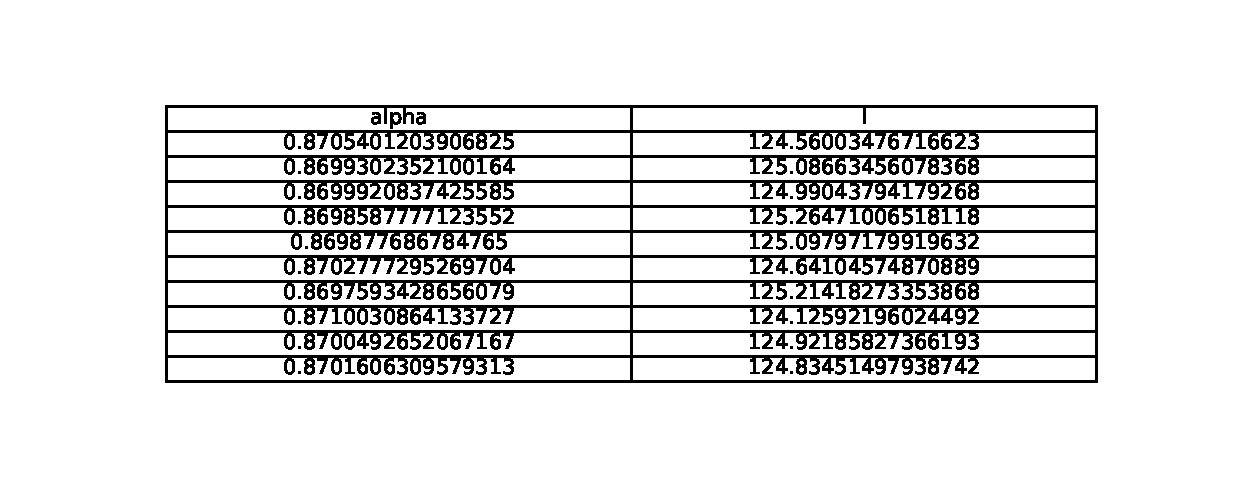
\includegraphics[width=1\textwidth]{data/ex6/Monte_Carlo.eps}
\end{figure}

Здесь альфа --- вероятность вычисленного значения попасть в доверительный интервал $[I - \varepsilon, I + \varepsilon],\, \varepsilon = 1$.

\subsubsection{Метод квадратур}

Посчитаем интеграл неоптимизированным способом. Для этого выберем число шагов сетки \(N = 5\) и проведем вычисления. Получим значение \(I = 116.39025860063605\).

Далее применим оптимизированный способ, учитывающий перестановочность аргументов функции. При \(N = 5\) получим тот же результат, что и в изначальном методе, что показывает их эквивалентность. Однако скорость этого метода намного выше. Выбрав \(N = 12\), получим значение \(I = 124.98912846401902\). Это намного более точная оценка истинного значения интеграла.



\section{Задание 7}
\subsection{Постановка задачи}
\begin{enumerate}
    \item Методом случайного поиска найти минимальное значение функции \(f\) на множестве $A = \{x_1, x_2: x_1^2 + x_2^2 \leqslant 1\}$, где

$$ f(x_1, x_2) = x_1^3 \sin(\frac{1}{x_1}) + 10 x_1 x_2^4 \cos(\frac{1}{x_2}),\quad x_1,x_2 \neq 0 $$

При $x_1 = 0$  или $x_2 = 0$ функция доопределяется по непрерывности.
\item Методом имитации отжига найти минимальное значение функции Розенброка \(g\)
в пространстве \(\mathbb{R}^2\), где 

$$g(x) = (x_1 - 1)^2 + 100 (x_2 - x_1^2)^2$$

\item Оценить точность и сравнить результаты со стандартными методами оптимизации.
\end{enumerate}

\subsection{Теоретические сведения}

\subsubsection{Метод случайного поиска}

В методе случайного поиска задается начальная точка $x$, после чего до выполнения критерия остановки повторяется следующее действие:

Выбирается случайная точка на окружности с центром в текущей точке. В классическом случае, рассматривающемся здесь, радиус окружности фиксирован. Если значение в новой точке меньше, чем в текущей, то текущая точка заменяется на новую, иначе точка не меняется.

В данном случае в качестве критерия остановки будет использоваться число итераций.

\subsubsection{Метод имитации обжига}

Название метода происходит от обжига в металлургии — это процесс, при котором металл постепенно охлаждатеся для изменения его физических свойств. Суть метода состоит в следующем:
\begin{enumerate}
    \item Выбираем начальное приближение (состояние системы) и температуру T (достаточно большую)
    \item На каждом шаге будем некоторым случайным способом выбирать соседнее состояние системы, и с некоторой вероятностью, зависящей от разницы функций в текущем и соседнем положениях (разнице энергий систем), перейдем в соседнее состояние. При этом понизим температуру по некоторому закону охлаждения.
\end{enumerate}

Таким образом, для реализации метода имитации отжига необходимо задать следующие элементы:
\begin{itemize}
    \item Метод генерации соседа как функцию от текущего положения системы $s_i = (x_i, y_i)$ и температуры $T_i$.
    \item Функцию вероятности перехода, зависящую от текущей температуры $T_i$ и разности значений минимизируемой функции $\Delta F = F(s_{i+1}) − F(s_i)$.
    \item Функцию понижения температуры системы \(T_{i+1}\) = $\mathcal{T}(T_i)$.
При этом, все эти функции являются параметрическими и вся сложность подбора сводится к отысканию оптимальных значений параметров для этих функций.
\end{itemize}


Будем использовать следующие семейства функций:
\begin{itemize}
    \item Функция выбора соседа — нормальная случайная величина со средним $(x_i, y_i)$ и дисперсией $\sigma^2 \dot T_i$
    \item Функция вероятности перехода $P = e^{-\frac{\Delta F_i}{T_i}}$
    \item Функция понижения температуры $T_{i + 1} = k T_i$
\end{itemize}

В качестве критериев качества модели будем рассматривать скорость сходимости (среднее число итераций для достаточно хорошей сходимости к минимуму), стабильность алгоритма и число переходов в другие точки.

\subsection{Результаты работы программы}

\subsubsection{Метод случайного поиска}

Применим метод случайного поиска для функции \(f\). Проведем по 5 вычислений для разных значений параметров:

\begin{figure}[H]

\includegraphics[width=1\textwidth]{data/ex7/ex1.eps}
\caption{Результаты работы метода случайного поиска (r = 0.1, R = 1, n_iter = 100000)}
\end{figure}
\begin{figure}[H]

\includegraphics[width=1\textwidth]{data/ex7/ex2.eps}
\caption{Результаты работы метода случайного поиска (r = 0.01, R = 1, n_iter = 100000)}
\end{figure}
\begin{figure}[H]

\includegraphics[width=1\textwidth]{data/ex7/ex3.eps}
\caption{Результаты работы метода случайного поиска (r = 0.001, R = 1, n_iter = 100000)}
\end{figure}
Как видно, точность метода увеличивается с уменьшением шага.

Провизуализируем путь алгоритма (начало в точке (0, 0)):

\begin{figure}[H]
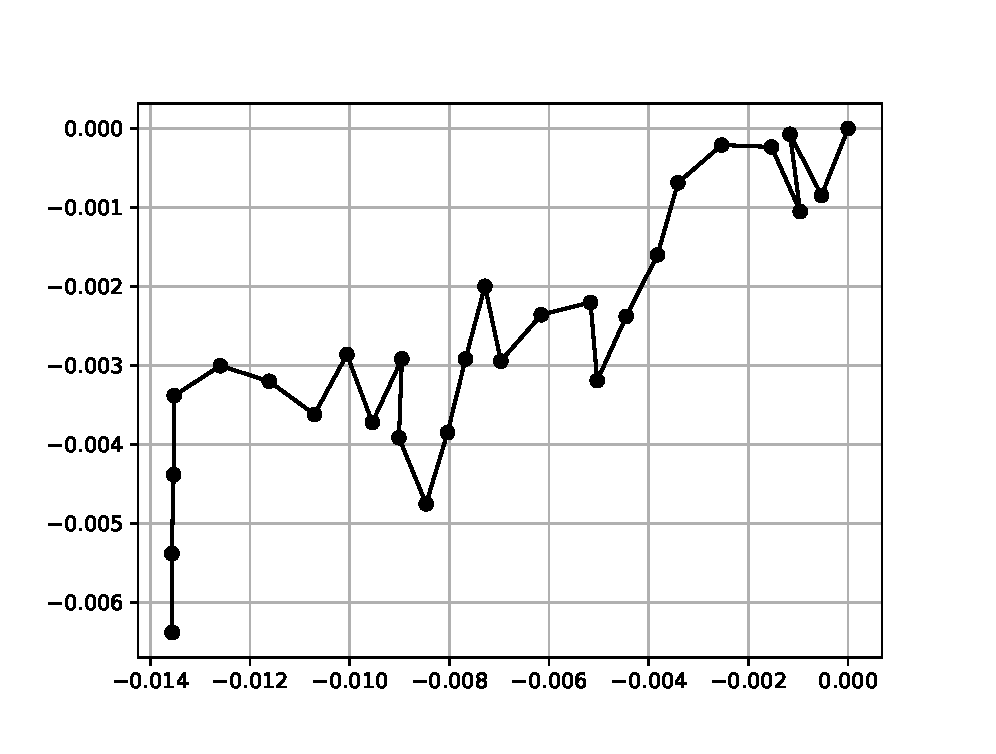
\includegraphics[width=1\textwidth]{data/ex7/ex_rs.eps}
\end{figure}

\subsubsection{Метод имитации обжига}

Выберем следующие параметры: \(x_0 = (0, 0), T_0 = 0.2, k = 0.98, \sigma = 1\), число итераций = 100.
Получим следующий результат: \(x = 0.7034296000028992, y = 0.49490954286193134, g(x, y) = 0.08795493030752062\).

Провизуализируем путь алгоритма:
\begin{figure}[H]
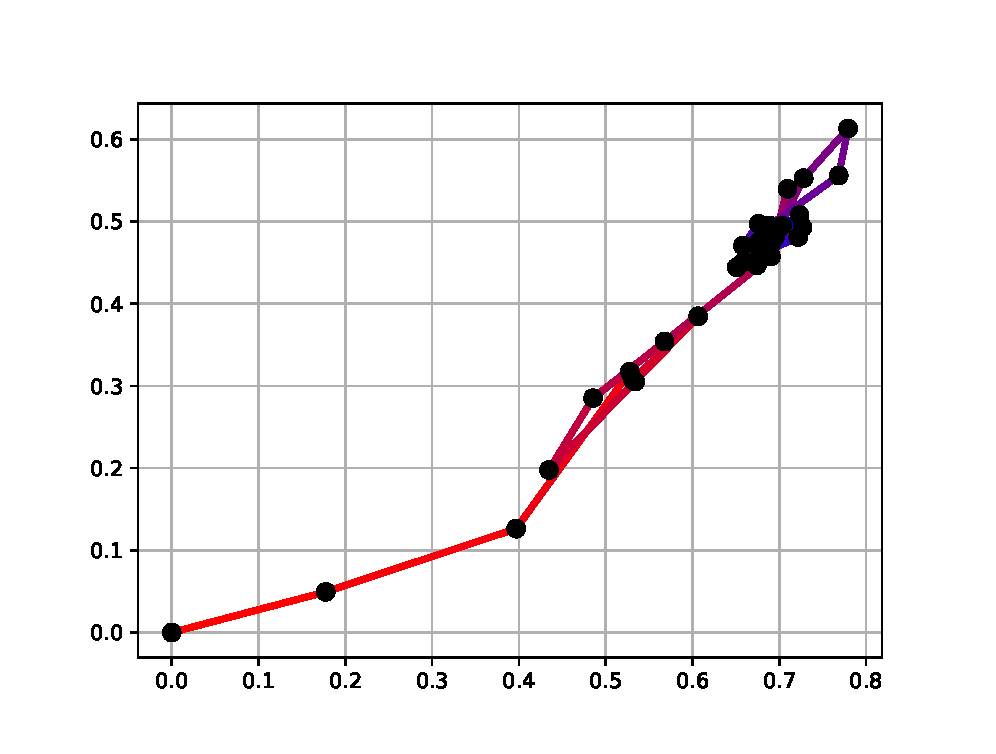
\includegraphics[width=1\textwidth]{data/ex7/ex_sa.eps}
\end{figure}

Определим лучшие параметры для разного числа итераций путем перебора по сетке и усреднения погрешности на нескольких испытаниях. Получим:


\begin{itemize}
    \item[] Best params for $n\_iter = 10$: $T_0 = 0.5$, $k = 0.95$, $\sigma = 0.5$, average function value: $4.763645708290797$, variance: $139.29890627450928$
    \item[] Best params for $n\_iter = 100$: $T_0 = 0.5$, $k = 0.95$, $\sigma = 0.5$, average function value: $0.2854564517173977$, variance: $0.03595942759493684$
    \item[] Best params for $n\_iter = 1000$: $T_0 = 1$, $k = 0.98$, $\sigma = 1$, average function value: $0.10025970964792115$, variance: $0.0031692159819085657$
    \item[] Best params for $n\_iter = 10000$: $T_0 = 1$, $k = 0.98$, $\sigma = 1$, average function value: $0.02402392504931519$, variance: $0$
    \item[] Total best function value: $0.017276779949925936$
\end{itemize}

\subsubsection{Сравнение со стандартными методами оптимизации}

Сравним работу случайных алгоритмов с классическим методом градиентного спуска. Градиент функции равен
$$ \nabla g(x_1, x_2) = \begin{bmatrix}
2 (x_1 - 1) - 400 (x_2 - x_1^2) x_1 \\
200 (x_2 - x_1^2) 
\end{bmatrix} $$
Проводя 1000 испытаний из случайных точек, получаем следующий результат:

\begin{itemize}
    \item[] Average function value: 7.718818230906625, variance: 268.73638080507664
    \item[] total best function value: 2.37784239079799e-08
\end{itemize}

Как видно, градиентный спуск здесь оказался нестабильным, однако в лучшем случае дает практически идеальный ответ.

Главное преимущество метода имитации обжига в том, что он не требует знания градиента функции. Если градиент невозможно вычислить аналитически, то придется либо считать численно (что сложно), либо пользоваться стохастическими методами, которые могут эффективно дать достаточно хорошее приближение решения (при правильно подобранных параметрах).

\section{Задание 8}
\subsection{Постановка задачи}
\begin{enumerate}
    \item Применить метод Монте-Карло к решению первой краевой задачи для двумерного уравнения Лапласа в единичном круге
    $$ \begin{cases}
\Delta u = 0,\, (x, y) \in D\\
u\vert_{\delta D} = f(x, y)\\
u \in C^2(D), f \in C(\delta D)\\
D = \{(x, y) \in \mathbb{R}^2: x^2 + y^2 \leqslant 1\}
\end{cases} $$ 
    \item Для функции \(f(x, y) = x^2 - y^2\) найти аналитическое решение и сравнить с полученным по методу Монте-Карло.
\end{enumerate}

\subsection{Теоретические сведения}

Для применения метода Монте-Карло введем двумерную сетку на прямоугольнике $[-1, 1]^2$ с $N^2$ точками: ${x_{ij} = (-1 + ih, -1 + jh)}, h = 2/N$. Так как никакие точки сетки не попадут в точности на границу круга, определим граничные точки как точки, у которых хотя бы один сосед из $\{x_{i-1, j}, x_{i+1,j}, x_{i,j-1}, x_{i,j+1}\}$ находится вне круга.

Построим разностную схему для данной задачи:
Для внутренних точек:
$$\frac{u_{i-1,j} - 2 u_{i, j} + u_{i+1, j}}{h^2} = 0$$
$$\frac{u_{i,j-1} - 2 u_{i, j} + u_{i, j+1}}{h^2} = 0$$
$$u_{i,j} = \frac{1}{4}\left(u_{i-1,j} + u_{i+1, j} + u_{i,j-1} + u_{i, j+1}\right)$$
Для граничных точек учтем краевое условие:
$$u_{i,j} = f(x_{i,j})$$

Метод Монте-Карло в данном случае состоит в следующем: Промоделируем случайное блуждание частицы во внутренней точке сетки. В каждый момент времени частица с равными вероятностями может перейти в одну из четырех соседних узлов сетки. Значение функции $u$ в точке $x_{i,j}$ будет равно матожиданию значения функции $f$ в точке, в которой траектория впервые достигнет границы. Для приближения матожидания будем многократно моделировать, а потом усреднять, движение частицы.

\subsection{Результаты работы программы}

Сравним численное решение с решением, полученным аналитически, для функции
$$f(x, y) = x^2 - y^2.$$
Заметим, что эта функция уже является гармонической ($\Delta f(x, y) = 2 - 2 \equiv 0$), поэтому она и будет решением задачи на всем круге. Построим графики:

\begin{figure}[H]
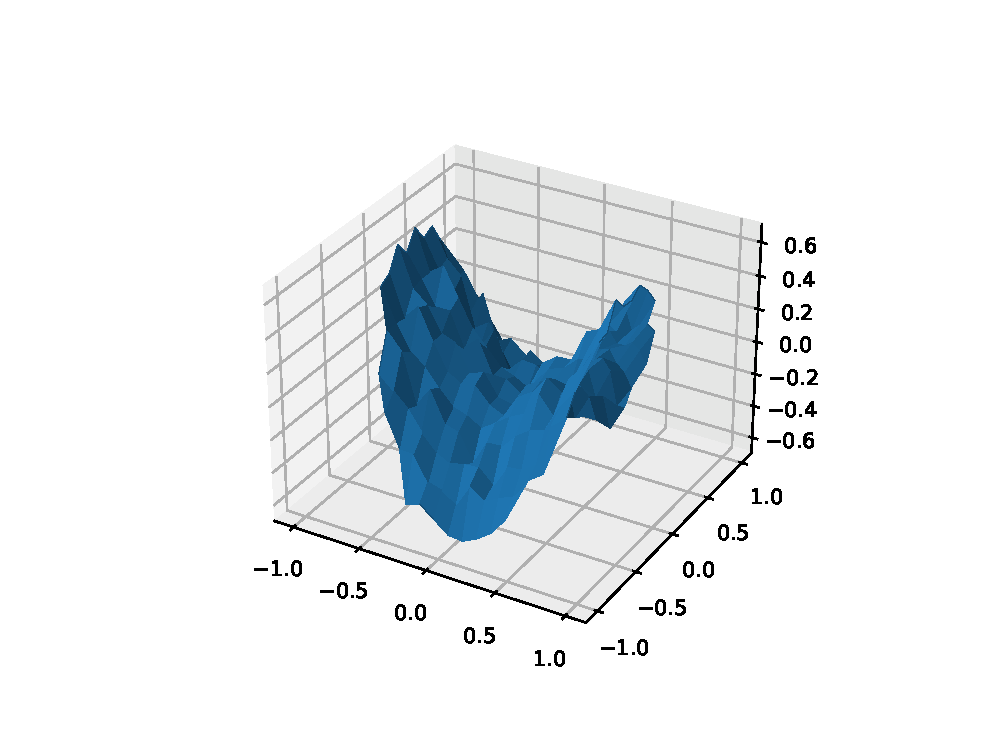
\includegraphics[width=1\textwidth]{data/ex8/mc.eps}
\caption{Решение методом Монте-Карло при \(N = 20\) и числе итераций = 100}
\end{figure}

\begin{figure}[H]
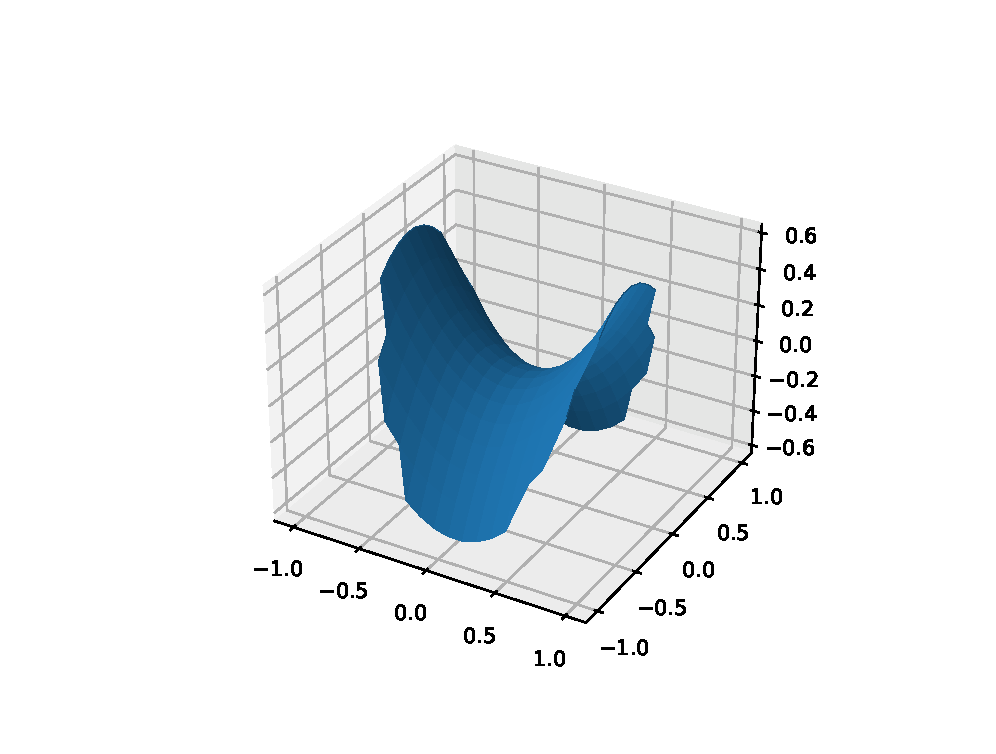
\includegraphics[width=0.9\textwidth]{data/ex8/anal.eps}
\caption{Аналитическое решение}
\end{figure}

\begin{figure}[H]

\includegraphics[width=0.9\textwidth]{data/ex8/err.eps}
\caption{Погрешность численного решения}
\end{figure}

\section{Задание 9}
\subsection{Постановка задачи}
Рассмотреть два вида гауссовских процессов:
\begin{itemize}
    \item Винеровский процесс \(W(t), t \in [0, 1], W(0) = 0\)
    \item Процесс Орнштейна–Уленбека \(X(t), t \in [0, 1], X(0) = X_0\), т.е. стационарный марковский гауссовский процесс. Начальные значения \(X_0\) следует выбирать случайным образом так, чтобы полученный процесс был стационарным.
\end{itemize}
Для данных процессов:
\begin{enumerate}
    \item Найти ковариационную функцию и переходные вероятности.
    \item Промоделировать независимые траектории процесса с данными переходными
    вероятностями методом добавления разбиения отрезка.
    \item Построить график траектории, не соединяя точки ломаной, с целью получения
    визуально непрерывной линии.
\end{enumerate}

\subsection{Теоретические сведения}

\subsubsection{Винеровский процесс}

Винеровским процесом $W(t),\, t \geqslant 0$, называется случайный процесс, для которого верно:
1. $W(0) = 0 \text{ п.н.}$
2. $W(t)$ --- $\text{ процесс с независимыми приращениями, то есть } \forall t_0, t_1, \dots, t_n \geqslant 0 \text{ таких, что } 0 = t_0 < t_1 < \dots < t_n, \text{ случайные величины } X_{t_0}, X_{t_1} - X_{t_0},\dots, X_{t_n} - X_{t_{n-1}} \text{ независимы}.$
3. $W(t) - W(s) \sim N(0, \sigma^2(t-s)), \forall 0 \leqslant s < t,$ где $N(0, \sigma^2(t-s))$ --- нормальное распределение со средним 0 и дисперсией $\sigma^2(t-s)$.

Винеровский процесс является марковским и гауссовским.

Найдем ковариационную функцию: Пусть $s \leqslant t$, тогда
$$\text{cov}(W(s), W(t)) = \mathbb{E}(W(s) - \mathbb{E}W(s))(W(t) - \mathbb{E}W(t)) = \mathbb{E}W(s)W(t) = $$
$$ = \mathbb{E}W(s)((W(t) - W(s)) + W(s)) = \mathbb{E}W(s)(W(t) - W(s)) + \mathbb{E} W^2(s).$$
В силу независимости приращений получаем, что случайные величины
$$W(s) = W(s) - W(0) \text{ и } W(t) - W(s)$$
независимы, поэтому
$$\mathbb{E}W(s)(W(t) - W(s)) = \mathbb{E}W(s) \cdot \mathbb{E}(W(t) - W(s)) = 0.$$
Таким образом,
$$\text{cov}(W(s), W(t)) = \mathbb{E}(W^2(s)) = \text{Var}(W^2(s)) = s\sigma^2.$$
В общем случае получаем
$$\text{cov}(W(s), W(t)) = \text{min}(s, t)\sigma^2.$$

Теперь рассмотрим переходные вероятности. Пусть, как и раньше, $0 \leqslant s < t$. Нас интересует условная плотность распределения:
$$p_{W(t)|W(s)}(y|x) = \frac{p_{W(s),W(t)}(x,y)}{p_{W(s)}(x)}$$
Заметим, что 
$$W(t) = W(t) - W(0) \sim N(0, \sigma^2t),\, W(s) = W(s) - W(0) \sim N(0, \sigma^2s),$$
поэтому случайный вектор $(W(s), W(t))$ имеет двумерное нормальное распределение с матожиданием $\mu = (0, 0)$ и ковариационной матрицей
$$\Sigma = \begin{bmatrix}
\text{cov}(W(s), W(s)) & \text{cov}(W(s), W(t))\\
\text{cov}(W(t), W(s)) & \text{cov}(W(t), W(t))\\
\end{bmatrix} = \sigma^2\begin{bmatrix}
s & s\\
s & t\\
\end{bmatrix},$$
$$\text{det}(\Sigma) = \sigma^4s(t-s),$$
$$\Sigma^{-1} = \frac{1}{\sigma^2s(t-s)}\begin{bmatrix}
t & -s\\
-s & s\\
\end{bmatrix}.$$
Таким образом,
$$
p_{W(s), W(t)}(x, y) = \frac{1}{2\pi \sigma^2 \sqrt{s(t-s)}}e^{-\frac{1}{2\sigma^2s(t-s)}\begin{bmatrix}x & y\end{bmatrix}\begin{bmatrix}
t & -s\\
-s & s\\
\end{bmatrix}\begin{bmatrix}x \\ y\end{bmatrix}} = $$
$$
 = \frac{1}{2\pi \sigma^2 \sqrt{s(t-s)}}e^{-\frac{1}{2\sigma^2s(t-s)}(tx^2 - 2sxy + sy^2)},
$$
$$p_{W(s)}(x) = \frac{1}{\sqrt{2\pi s}\sigma}e^{-\frac{1}{2}\frac{x^2}{\sigma^2s}},$$
и
$$
p_{W(t)|W(s)}(y|x) = \frac{\sqrt{2\pi s}\sigma}{2\pi \sigma^2 \sqrt{s(t-s)}}e^{-\frac{1}{2\sigma^2s(t-s)}(tx^2 - 2sxy + sy^2) + \frac{1}{2}\frac{x^2}{\sigma^2s}} = 
$$
$$ = \frac{1}{\sqrt{2\pi(t-s)} \sigma}e^{-\frac{1}{2\sigma^2s(t-s)}(sx^2 - 2sxy + sy^2)} = 
\frac{1}{\sqrt{2\pi(t-s)} \sigma}e^{-\frac{1}{2\sigma^2(t-s)}(y - x)^2}.
$$
Значит, 
$$(W(t)|W(s)=x) \sim N(x, \sigma^2(t - s))$$

Для метода разбиения отрезка нам также понадобится условная вероятность для средней точки отрезка при известных крайних. Пусть $0 \leqslant t_1 < t_2 < t_3$. Тогда
$$p_{W(t_2)|W(t_1),W(t_3)}(y|x,z) = \frac{p_{W(t_1),W(t_2),W(t_3)}(x,y,z)}{p_{W(t_1),W(t_3)}(x,z)},$$
$$\Sigma_{t_1, t_2, t_3} = \sigma^2\begin{bmatrix}
t_1 & t_1 & t_1\\
t_1 & t_2 & t_2\\
t_1 & t_2 & t_3\\
\end{bmatrix},$$
$$\text{det}(\Sigma_{t_1, t_2, t_3}) = \sigma^6t_1(t_2 - t_1)(t_3 - t_2),$$
$$\Sigma_{t_1, t_2, t_3}^{-1} = \frac{1}{\sigma^2t_1(t_2 - t_1)(t_3 - t_2)}\begin{bmatrix}
t_2(t_3 - t_2) & t_1(t_2 - t_3) & 0\\
t_1(t_2 - t_3) & t_1(t_3 - t_1) & t_1(t_1 - t_2)\\
0 & t_1(t_1 - t_2) & t_1(t_2 - t_1)\\
\end{bmatrix},$$
$$p_{W(t_1),W(t_2),W(t_3)}(x,y,z) = $$
$$ = \frac{1}{\left(2\pi\sigma^2\right)^{\frac{3}{2}}\sqrt{t_1(t_2 - t_1)(t_3 - t_2)}}e^{-\frac{1}{2\sigma^2t_1(t_2 - t_1)(t_3 - t_2)}\begin{bmatrix}x & y & z\end{bmatrix}\begin{bmatrix}
t_2(t_3 - t_2) & t_1(t_2 - t_3) & 0\\
t_1(t_2 - t_3) & t_1(t_3 - t_1) & t_1(t_1 - t_2)\\
0 & t_1(t_1 - t_2) & t_1(t_2 - t_1)\\
\end{bmatrix}\begin{bmatrix}x \\ y \\ z\end{bmatrix}}.$$

В методе разбиения отрезка мы будем брать $t_2 = \frac{t_1 + t_3}{2}$, поэтому
$$\text{det}(\Sigma_{t_1, t_2, t_3}) = \sigma^6t_1(\frac{t_1 + t_3}{2} - t_1)(t_3 - \frac{t_1 + t_3}{2}) = \sigma^6t_1\left(\frac{t_3 - t_1}{2}\right)^2,$$
$$\Sigma_{t_1, t_2, t_3}^{-1} = \frac{1}{\sigma^2t_1\left(\frac{t_3 - t_1}{2}\right)^2}\begin{bmatrix}
\frac{t_1 + t_3}{2}\frac{t_3 - t_1}{2} & t_1\frac{t_1 - t_3}{2} & 0\\
t_1\frac{t_1 - t_3}{2} & t_1(t_3 - t_1) & t_1\frac{t_1 - t_3}{2}\\
0 & t_1\frac{t_1 - t_3}{2} & t_1\frac{t_3 - t_1}{2}\\
\end{bmatrix},$$
$$p_{W(t_1),W(t_2),W(t_3)}(x,y,z) = \frac{1}{\left(2\pi\sigma^2\right)^{\frac{3}{2}}\sqrt{t_1}\frac{t_3 - t_1}{2}}e^{-\frac{2}{\sigma^2t_1(t_3 - t_1)^2}\begin{bmatrix}x & y & z\end{bmatrix}\begin{bmatrix}
\frac{t_3^2 - t_1^2}{4} & t_1\frac{t_1 - t_3}{2} & 0\\
t_1\frac{t_1 - t_3}{2} & t_1(t_3 - t_1) & t_1\frac{t_1 - t_3}{2}\\
0 & t_1\frac{t_1 - t_3}{2} & t_1\frac{t_3 - t_1}{2}\\
\end{bmatrix}\begin{bmatrix}x \\ y \\ z\end{bmatrix}} = $$
$$
 = \frac{1}{\pi^{\frac{3}{2}}\sigma^3\sqrt{2 t_1}(t_3 - t_1)}e^{-\frac{2}{\sigma^2t_1(t_3 - t_1)^2}\left(\frac{t_3^2 - t_1^2}{4}x^2 + y(x + z - y)t_1(t_1 - t_3) + t_1\frac{t_3 - t_1}{2}z^2\right)},
$$
$$
p_{W(t_1), W(t_3)}(x, z) = \frac{1}{2\pi \sigma^2 \sqrt{t_1(t_3-t_1)}}e^{-\frac{1}{2\sigma^2t_1(t_3-t_1)}(t_3x^2 - 2t_1xz + t_1z^2)},
$$
$$p_{W(t_2)|W(t_1),W(t_3)}(y|x,z) = $$
$$ =\frac{2\pi \sigma^2 \sqrt{t_1(t_3-t_1)}}{\pi^{\frac{3}{2}}\sigma^3\sqrt{2 t_1}(t_3 - t_1)}e^{-\frac{2}{\sigma^2t_1(t_3 - t_1)^2}\left(\frac{t_3^2 - t_1^2}{4}x^2 + y(x + z - y)t_1(t_1 - t_3) + t_1\frac{t_3 - t_1}{2}z^2\right) + \frac{1}{2\sigma^2t_1(t_3-t_1)}(t_3x^2 - 2t_1xz + t_1z^2)}.$$
$$ -\frac{2}{\sigma^2t_1(t_3 - t_1)^2}\left(\frac{t_3^2 - t_1^2}{4}x^2 + y(x + z - y)t_1(t_1 - t_3) + t_1\frac{t_3 - t_1}{2}z^2\right) + \frac{1}{2\sigma^2t_1(t_3-t_1)}(t_3x^2 - 2t_1xz + t_1z^2) = $$
$$ = \frac{1}{2\sigma^2t_1(t_3 - t_1)^2}(-(t_3 - t_1)(t_3 + t_1)x^2 + 4t_1(t_3 - t_1)y(x + z - y) - $$
$$ - 2t_1(t_3 - t_1)z^2 + t_3(t_3 - t_1)x^2 - 2t_1(t_3 - t_1)xz + t_1(t_3 - t_1)z^2) = $$
$$ = \frac{1}{2\sigma^2t_1(t_3 - t_1)^2}(-4t_1(t_3 - t_1)y^2 + 4t_1(t_3 - t_1)(x + z)y + (-(t_3 - t_1)(t_3 + t_1)x^2 -$$
$$ - 2t_1(t_3 - t_1)z^2 + t_3(t_3 - t_1)x^2 - 2t_1(t_3 - t_1)xz + t_1(t_3 - t_1)z^2)) = $$
$$ = -\frac{1}{2\sigma^2(t_3 - t_1)}\left(4y^2 - 4y(x + z) + (x^2 + 2xz + z^2)\right) = -\frac{2}{\sigma^2(t_3 - t_1)}\left(y - \frac{x + z}{2}\right)^2 \Rightarrow$$
$$ \Rightarrow p_{W(t_2)|W(t_1),W(t_3)}(y|x,z) = \frac{1}{\sigma\sqrt{\pi \frac{t_3-t_1}{2}}}e^{-\frac{2}{\sigma^2(t_3 - t_1)}\left(y - \frac{x + z}{2}\right)^2} = \frac{1}{\sigma\sqrt{2\pi \frac{t_3-t_1}{4}}}e^{-\frac{1}{2\sigma^2\frac{t_3 - t_1}{4}}\left(y - \frac{x + z}{2}\right)^2}.$$
Таким образом, получаем, что 
$$(W(t_2)|W(t_1)=x,W(t_3)=z) \sim N(\frac{x + z}{2}, \sigma^2\frac{t_3 - t_1}{4}).$$

\subsubsection{Процесс Орнштейна-Уленбека}

Процесс Орнштейна-Уленбека $X(t), t \in [0, 1], X(0) = X_0$ --- единственный нетривиальный гауссовский процесс, являющийся стационарным и обладающий марковским свойством. Начальные значения $X_0$ выбираются случайным образом так, чтобы процесс был стационарным. Для этого необходимо и достаточно, чтобы $X_0 \sim N(\mu, \sigma^2)$

Выведем ковариационную функцию процесса. Пусть $0 \leqslant s < t$. Без ограничения общности, рассмотрим процессы с $\mu = 0$. В силу стационарности процесса,
$$\text{cov}(X(s), X(t)) = \text{cov}(X(0), X(t-s)) = K(t-s).$$
Рассмотрим условное матожидание $\mathbb{E}(X(t + h)|X(t))$. В силу того, что $X(t + h)$ и $X(t)$ --- совместно гауссовские случайные величины,
$$\mathbb{E}(X(t + h)|X(t)) = \frac{\text{cov}(X(t + h), X(t))}{\text{Var(X(t))}}X(t) = \frac{K(h)}{\sigma^2}X(t).$$
Теперь посчитаем величину $\mathbb{E}(X(t + h + s)|X(t))$ двумя способами. С одной стороны,
$$\mathbb{E}(X(t + h + s)|X(t)) = \frac{K(h + s)}{\sigma^2}X(t).$$
С другой же, используя марковское свойство и свойства условного матожидания,
$$\mathbb{E}(X(t + h + s)|X(t)) = \mathbb{E}(\mathbb{E}(X(t + h + s)|X(t + h))|X(t)) = \mathbb{E}(\frac{K(s)}{\sigma^2}X(t + h)|X(t)) = \frac{K(s)}{\sigma^2}\frac{K(h)}{\sigma^2}X(t).$$
Таким образом,
$$\frac{K(h + s)}{\sigma^2}X(t) = \frac{K(s)}{\sigma^2}\frac{K(h)}{\sigma^2}X(t),$$
$$\frac{K(h + s)}{\sigma^2} = \frac{K(s)}{\sigma^2}\frac{K(h)}{\sigma^2}.$$
В силу непрерывности решений, получаем, что уравнение имеет единственное решение
$$\frac{K(h)}{\sigma^2} = e^{-\theta h}$$
для некоторой константы $\theta$. В силу того, что корреляция должна быть ограничена, получаем, что $\theta > 0$. В общем случае, имеем
$$K(h) = \sigma^2 e^{\theta\vert h \vert}$$

Процесс нахождения переходных вероятностей аналогичен случаю винеровского процесса, в котором нужно заменить ковариационную функцию на соответствующую функцию для процесса Орнштейна-Уленбека, и учесть ненулевое матожидание. В итоге получим, что если $X_0 \sim N(\mu, \sigma^2)$, то
$$(X(t) | X_0 = x) \sim N(\mu + (x - \mu)e^{-\theta t}, \sigma^2(1 - e^{-2 \theta t})),$$
$$(X(t_2) | X(t_1) = x,X(t_3) = z) \sim N(\frac{x + z}{e^{\theta h} + e^{-\theta h}}, \sigma^2\frac{e^{2 \theta h} - 1}{e^{2 \theta h} + 1}),$$
где $t \geqslant 0,\, t_1 < t_3,\, t_2 = \frac{t_1 + t_3}{2},\, h = \frac{t_3 - t_1}{2}$.

\subsection{Результаты работы программы}

Промоделируем процессы, используя метод разбиения отрезка. Для этого сначала сгенерируем величину в нулевой момент времени из безусловного распределения, потом в момент $t = 1$ при условии начального значения, а далее будем делить отрезки пополам и генерировать значения посередине при условии значений на концах.

Начнем с винеровского процесса: выберем \(\sigma = 1\), глубину разбиения (то есть число раз, которое мы будем делить отрезки пополам), равную 15.

\begin{figure}[H]
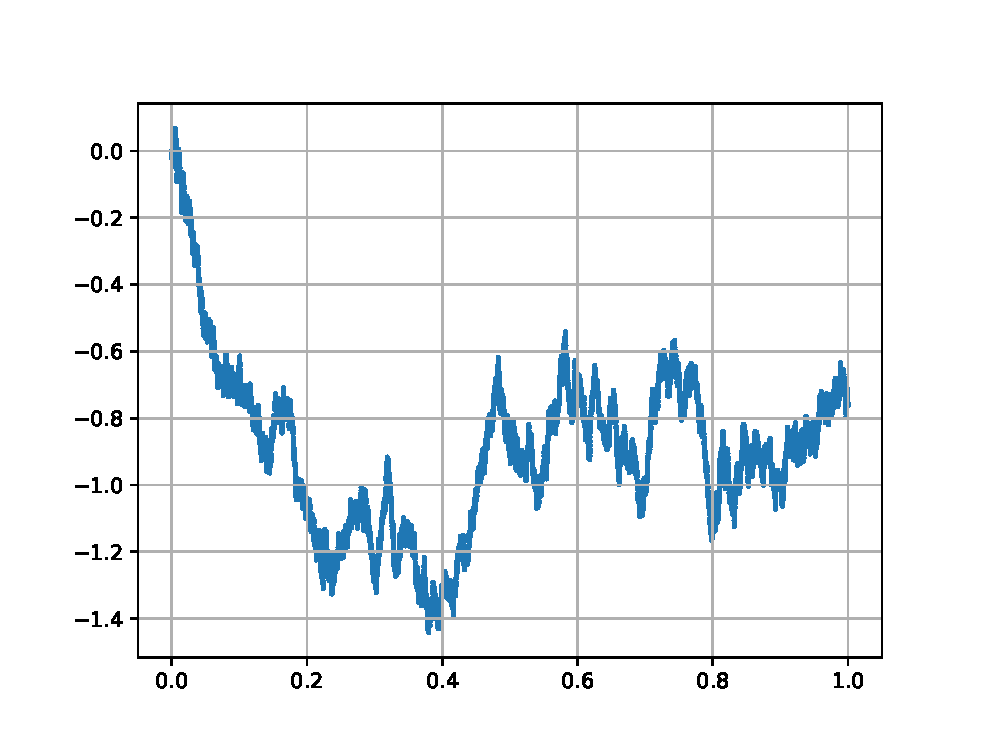
\includegraphics[width=1\textwidth]{data/ex9/Wiener.eps}
\caption{Решение методом Монте-Карло при \(N = 20\) и числе итераций = 100}
\end{figure}

Для процесса Орнштейна-Уленбека рассмотрим разные наборы параметров:

\begin{figure}[H]
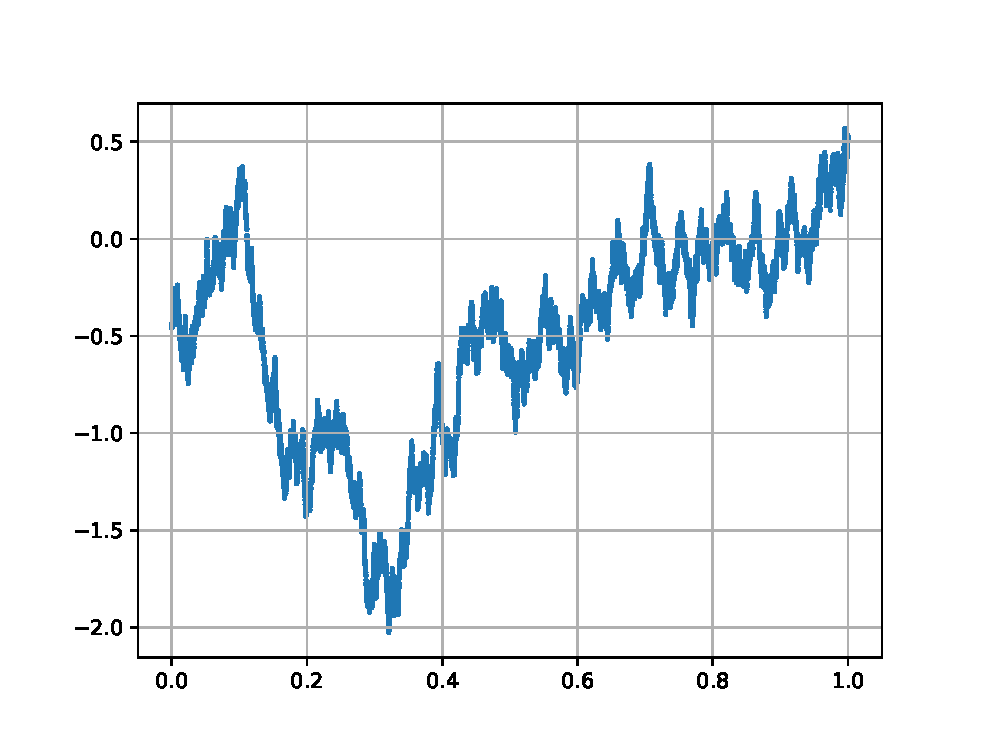
\includegraphics[width=1\textwidth]{data/ex9/OU1.eps}
\caption{\(\sigma = 1, \mu = 0, \theta = 1, \text{depth} = 15\)}
\end{figure}

\begin{figure}[H]
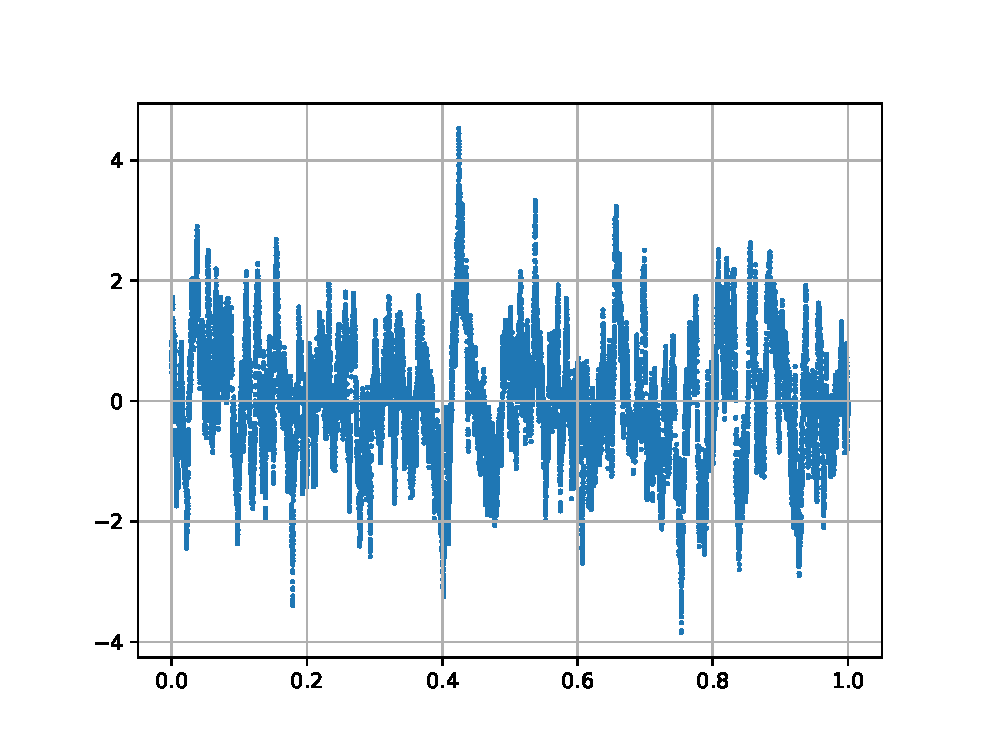
\includegraphics[width=1\textwidth]{data/ex9/OU2.eps}
\caption{\(\sigma = 1, \mu = 0, \theta = 100, \text{depth} = 15\)}
\end{figure}

\begin{figure}[H]
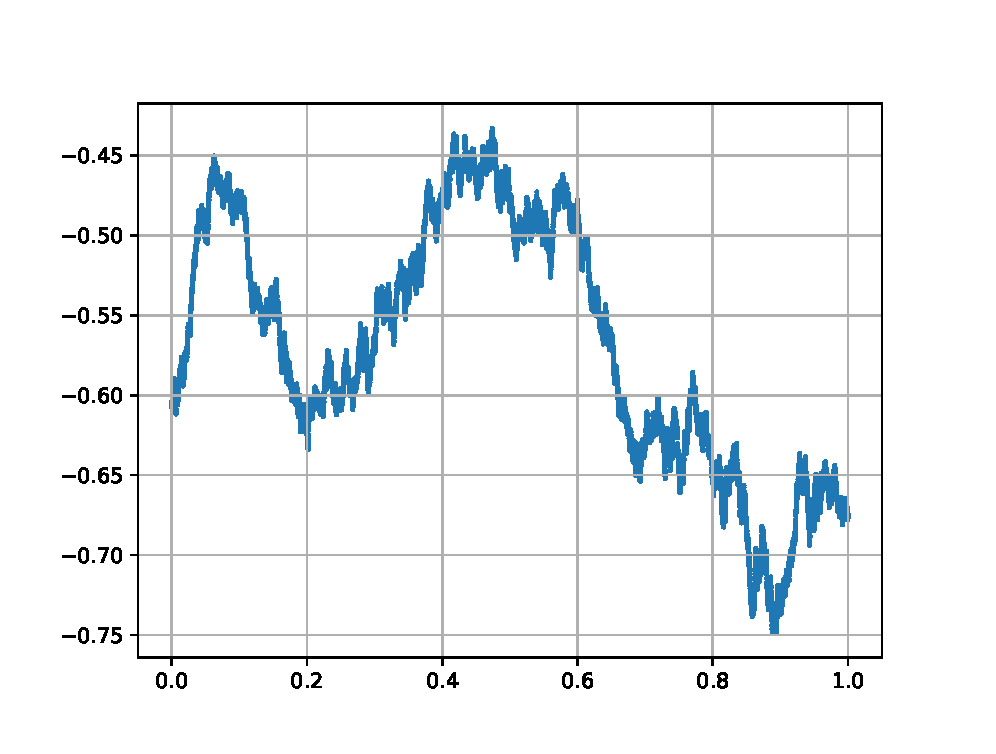
\includegraphics[width=1\textwidth]{data/ex9/OU3.eps}
\caption{\(\sigma = 1, \mu = 0, \theta = 0.01, \text{depth} = 15\)}
\end{figure}

\section{Задание 10}
\subsection{Постановка задачи}
Произвести фильтрацию одномерного процесса Орнштейна-Уленбека:
\begin{enumerate}
    \item Используя генератор белого шума, добавить к реализации процесса Орнштейна-Уленбека случайную ошибку с заранее известной дисперсией.
    \item При помощи одномерного фильтра Калмана оценить траекторию процесса по
    зашумленному сигналу, считая известными параметры шума и процесса.
    \item Рассмотреть следующие виды шума:
    \begin{enumerate}
        \item Гауссов
        \item Коши (шум имеет распределение Коши)
    \end{enumerate}
\end{enumerate}

\subsection{Теоретические сведения}

\subsubsection{Фильтр Калмана}

Рассмотрим сначала нормально распределенный шум. Одномерный фильтр Каллмана рассматривается для системы вида
$$x_{n + 1} = a x_n + \nu_n,\ \text{i.i.d.}\, \nu_n \sim N(0, q),\ x_1 \sim N(0, \sigma^2),$$
$$y_n = x_n + \varepsilon_n,\ \text{i.i.d.}\, \varepsilon_n \sim N(0, r).$$
Значение дисперсии шума $r$ считается изветным еще на этапе генерации этого шума.

Для определения коэффициентов уравнения динамики необходимо приравнять
теоретические значения ковариационной матрицы процесса Орнштейна-Уленбека в
точках $t_n$ и $t_{n+1}$ c соответствующими значениями динамической системы, то есть
решить систему уравнений относительно неизвестных коэффициентов $a$ и $q$ через известные $\sigma$ и $\theta$:
$$\begin{cases}
\sigma^2 = R(t_n, t_n) = \text{Var}(x_n)\\
\sigma^2e^{-\theta(t_{n+1} - t_n)} = R(t_n, t_n+1) = \text{cov}(x_n, x_{n + 1}) = a \text{Var}(x_n)\\
\sigma^2 = R(t_{n+1}, t_{n+1}) - \text{Var}(x_{n+1}) = a^2 \text{Var}(x_n) + q
\end{cases}$$
При фильтрации значение оригинального процесса $x_n$ неизвестно. Вместо него доступен наблюдаемый зашумленный сигнал $y_n$.

Рассмотрим работу фильтра Калмана в произвольный момент времени $t$. Пусть $\hat{x}_{n|n}$ --- прогноз значения $x_n$ при известных $y_1,\dots y_n$, $\hat{x}_{n|n}$ --- экстраполяция процесса на следующий шаг в соответствии с динамической системой. Через $p_{n|n}$ будем обозначать дисперсию ошибки фильтрации на n-м шаге, через $p_{n|n−1}$ — прогнозируемую на следующем шаге дисперсию. Тогда каждый шаг заключается в следующем:
1. Прогнозируем значение процесса и дисперсию ошибки
$$\hat{x}_{n|n-1} = a\hat{x}_{n-1|n-1},\ p_{n|n-1} = a^2p_{n-1|n-1} + q$$
2. Вычисляем разницу между наблюдаемым процессом и прогнозом и коэффициент усиления Калмана
$$\delta_n = y_n - \hat{x}_{n|n-1},\ k_n = \frac{p_{n|n-1}}{p_{n|n-1} + r}$$
3. В качестве результата фильтрации берем выпуклую комбинацию наблюдаемого
и предсказанного значения
$$\hat{x}_{n|n} = \hat{x}_{n|n-1} + k_n \delta_n,\ p_{n|n} = (1 - k_n)p_{n|n-1}$$

Поскольку рассматривается линейный фильтр гауссовского процесса с гауссовским шумом, ошибка фильтрации будет иметь нормальное распределение, а доверительный интервал с уровнем доверия $\alpha$ будет иметь вид
$$[\hat{x}_{n|n} - \Delta, \hat{x}_{n|n} + \Delta],\ \Delta = -\sqrt{p_{n|n}}\Phi^{-1}\left(\frac{\alpha}{2}\right)$$
Обозначим $h = t_{n + 1} - t_n$. Из системы легко получаем, что
$$a = e^{-\theta h},\, q = \sigma^2(1 - a^2) = \sigma^2(1 - e^{-2\theta h})$$

При рассмотрении шума, распределенного по Коши, возникает следующая проблема: у такой случайной величины не существует дисперсии, поэтому невозмоно сделать второй шаг. Фильтр Калмана не подходит для такой задачи.

\subsection{Результаты работы программы}

Будем рассматривать нормально распределенный шум.

\begin{figure}[H]
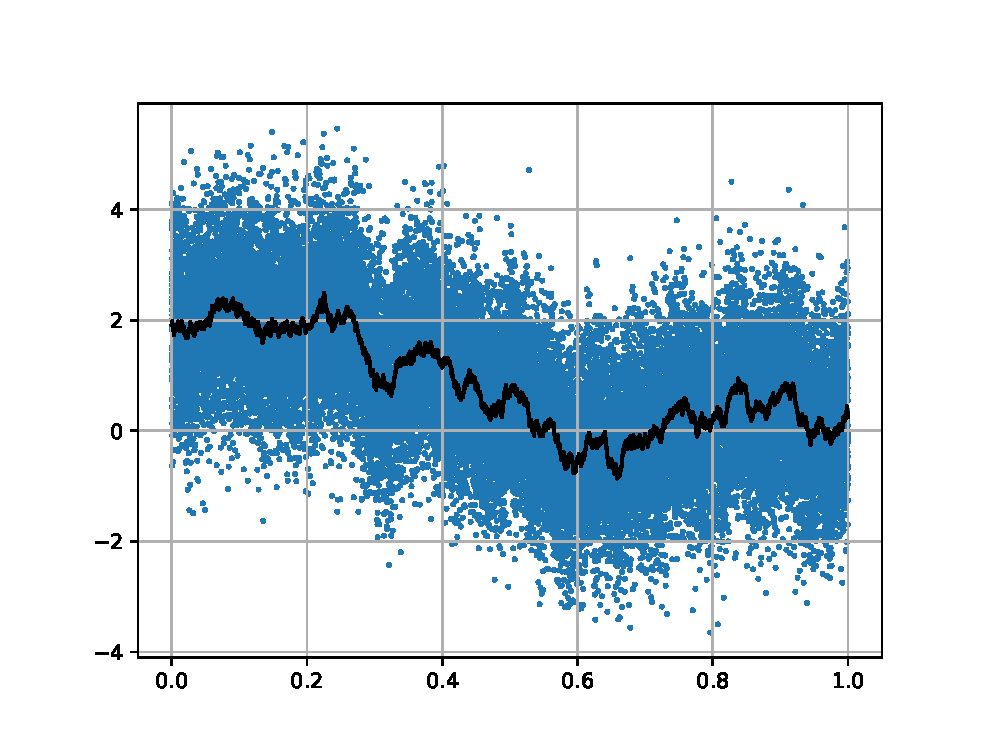
\includegraphics[width=1\textwidth]{data/ex10/noised.eps}
\caption{Зашумленный процесс Орнштейна-Уленбека \(\mu = 0,\, \sigma = 1,\, \theta = 1,\, \text{depth} = 15,\, \text{дисперсия шума } r = 1\)}
\end{figure}

\begin{figure}[H]
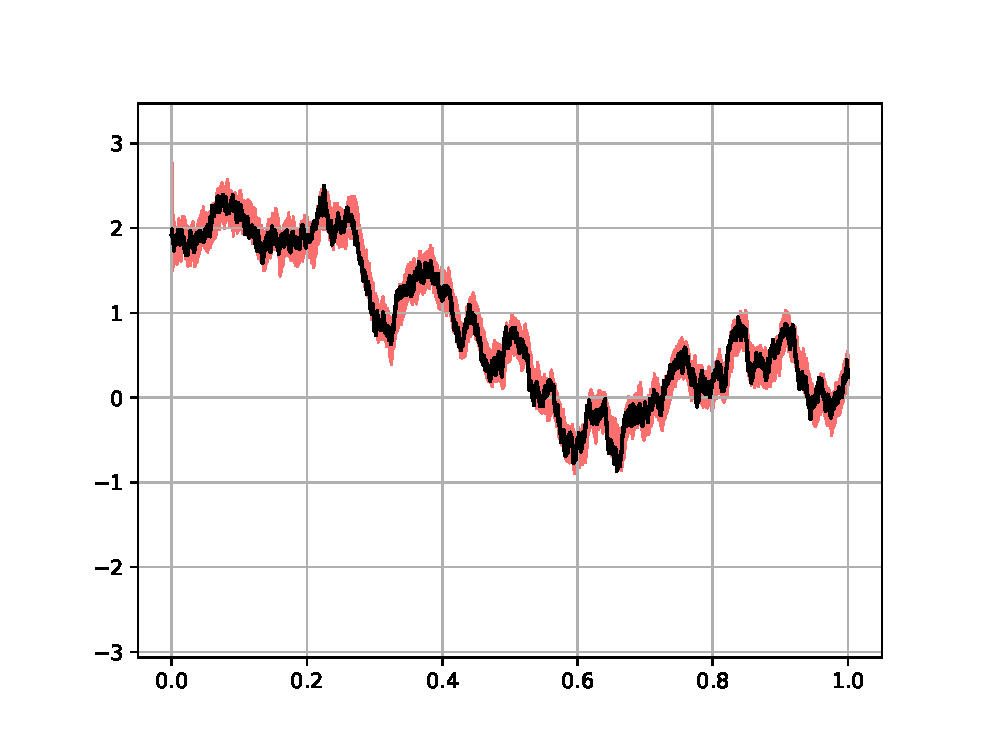
\includegraphics[width=1\textwidth]{data/ex10/filtered.eps}
\caption{Истинная тракетория (черный) и результат работы фильтра Калмана --- доверительные интервалы с уровнем доверия \(\alpha = 0.95\)}
\end{figure}

\begin{figure}[H]
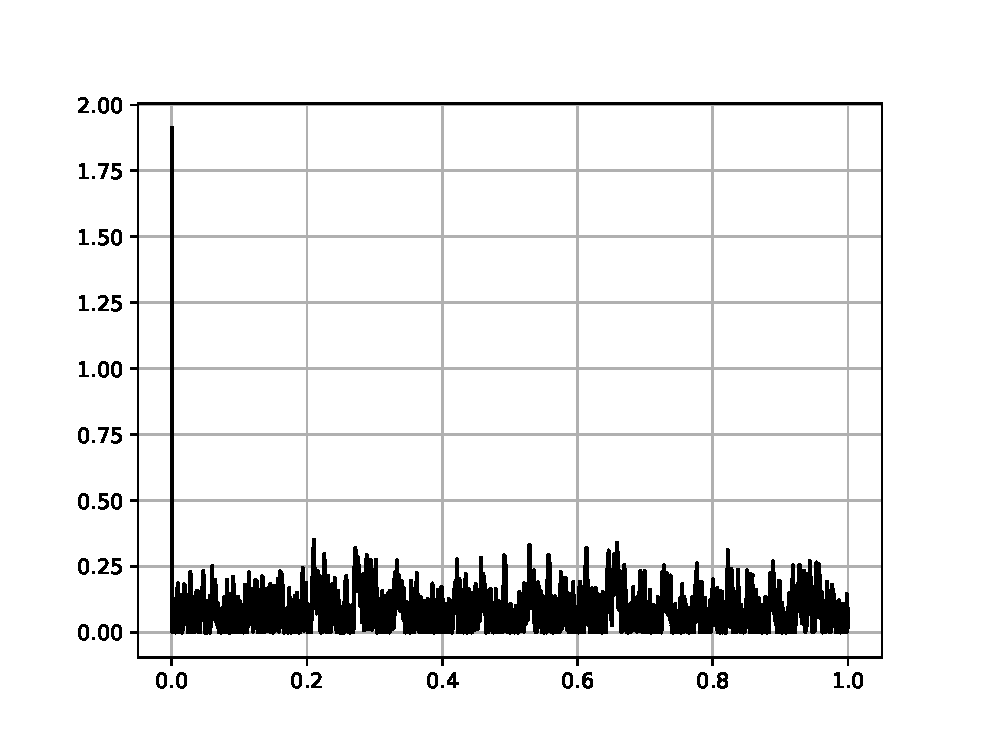
\includegraphics[width=1\textwidth]{data/ex10/err.eps}
\caption{Отклонение предсказанного решения от истинного}
\end{figure}

\section{Задание 11}
\subsection{Постановка задачи}
Построить двумерное пуассоновское поле, отвечающее сложному пуассоновскому процессу:

\begin{enumerate}
    \item Система массового обслуживания. Первая координата поля — время поступления заявки в СМО (распределенное равномерно), а вторая — время обслуживания заявки (распределение \(\chi^2\) с десятью степенями свободы).
    \item Система массового обслуживания с циклической интенсивностью \(\lambda_0(1 + cos(t))\) и
единичными скачками. При помощи метода Льюиса и Шедлеара, свести задачу
моделирования неоднородного пуассоновского процесса к моделированию двумерного пуассоновского поля, где первая координата распределена равномерно,
а вторая имеет распределение Бернулли.
    \item Работа страховой компании: первая координата — момент наступления страхового случая (равномерное распределение), вторая — величина ущерба (распределение Парето). Поступление капитала считать линейным по времени со
скоростью \(c > 0\), начальный капитал \(W > 0\).

\end{enumerate}

\subsection{Теоретические сведения}

\subsubsection{Система массового обслуживания}

Первая координата поля — время поступления заявки в СМО (распределенное равномерно), а вторая — время обслуживания заявки (распределение $\chi^2$
с десятью степенями свободы).

Пусть первая координата распределена равномерно на отрезке $[0, T]$. В силу пуассоновости поля, число заявок за время T имеет пуассоновское распределение: $N \sim \text{Pois}(\lambda T)$, где $\lambda$ --- интенсивность поступления заявок.

Пусть $t_1, \dots, t_N$ --- н.о.р.с.в. --- времена поступления заявок, $t_i \sim U[0, T], i = \overline{1,10}$;  $\tau_1, \dots, \tau_N$ --- н.о.р.с.в. --- длительности обработки заявок, $\tau_i \sim \chi^2(10), i = \overline{1,10}$.

Для моделирования поля будем сначала моделировать величину $N$, а потом --- $t_i$ и $\tau_i,\, i = \overline{1,N}$.

\subsubsection{Система массового обслуживания с циклической интенсивностью}

Система массового обслуживания с циклической интенсивностью $\lambda(t) = \lambda_0(1 + \text{cos}(t))$ и единичными скачками. При помощи метода Льюиса и Шедлера, свести задачу моделирования неоднородного пуассоновского процесса к моделированию двумерного пуассоновского поля, где первая координата распределена равномерно, а вторая имеет распределение Бернулли.

Идея метода Льюиса и Шедлера заключается в следующем: Промоделируем пуассоновский процесс с максимальной интенсивностью, а затем отбросим часть точек с вероятностью, соответствующей интенсивности процесса в тот момент времени. В данном случае $0 \leqslant \lambda(t) \leqslant 2 \lambda_0$, поэтому будем моделировать процесс с постоянной интенсивностью $\lambda_{max} = 2 \lambda_0$. После этого будем удалять каждую точку с вероятностью $p(t) = 1 - \frac{\lambda(t)}{\lambda_{max}}$.

\subsubsection{Работа страховой компании}

Работа страховой компании: первая координата — момент наступления страхового случая (равномерное распределение), вторая — величина ущерба (распределение Парето). Поступление капитала считать линейным по времени со скоростью $c > 0$, начальный капитал $W_0 > 0$.

Распределение Парето --- семейство абсолютно непрерывных распределений с параметрами $x_m$ и $k$, функция распределения которого имеет вид
$$F_X(x) = \begin{cases} 1 - \left(\frac{x_m}{x}\right)^k,\ x \geqslant x_m, \\ 0,\ \text{иначе,}\end{cases}$$
а плотность распределения:
$$f_X(x) = \begin{cases} \frac{kx_m^k}{x^{k+1}},\ x \geqslant x_m, \\ 0,\ \text{иначе.}\end{cases}$$

Модель страховой компании состоит в следующем: капитал линейно растет со скоростью $c$ при этом в случайные моменты времени (имеющие пуассоновское распределение) происходит страховой случай, и из капитала вычитается сумма $X \sim P(x_m, k)$. При этом капитал не может быть отрицательным, то есть если капитал достигает нуля, то происходит банкротство, и далее он тождественно равен нулю. Таким образом, капитал имеет значение
$$W(t) = W_0 + ct - \sum_{i = 1}^{N(t)}X_i,$$
где $N(t)$ --- пуассоновский процесс с параметром $\lambda, X_i \sim P(x_m, k)$.

Исследуем поведение капитала со временем. Для этого найдем матожидание $\mathbb{E}W(t)$. Известно, что для распределения Парето $\mathbb{E}X = \frac{kx_m}{k - 1}$ (при $k > 1$), поэтому
$$\mathbb{E}W(t) = \mathbb{E}(W_0 + ct - \sum_{i = 1}^{N(t)}X_i) = W_0 + ct - \lambda t \frac{kx_m}{k - 1} = W_0 + t\left(c - \lambda \frac{kx_m}{k - 1}\right).$$
Таким образом, при $c - \lambda \frac{kx_m}{k - 1} > 0$ капитал будет в среднем возрастать, а при $c - \lambda \frac{kx_m}{k - 1} < 0$ --- убывать.

Будем генерировать распределение Парето путем обращения функции распределения: $F_X^{-1}(U) \sim X$, где $U \sim U[0, 1]$. Найдем обратную функцию распределения:
$$y = 1 - \left(\frac{x_m}{x}\right)^k$$
$$\frac{x_m}{x} = (1 - y)^{\frac{1}{k}}$$
$$x = F_X^{-1}(y) = x_m (1 - y)^{-\frac{1}{k}}$$

\subsection{Результаты работы программы}

\subsubsection{Система массового обслуживания}

\begin{figure}[H]
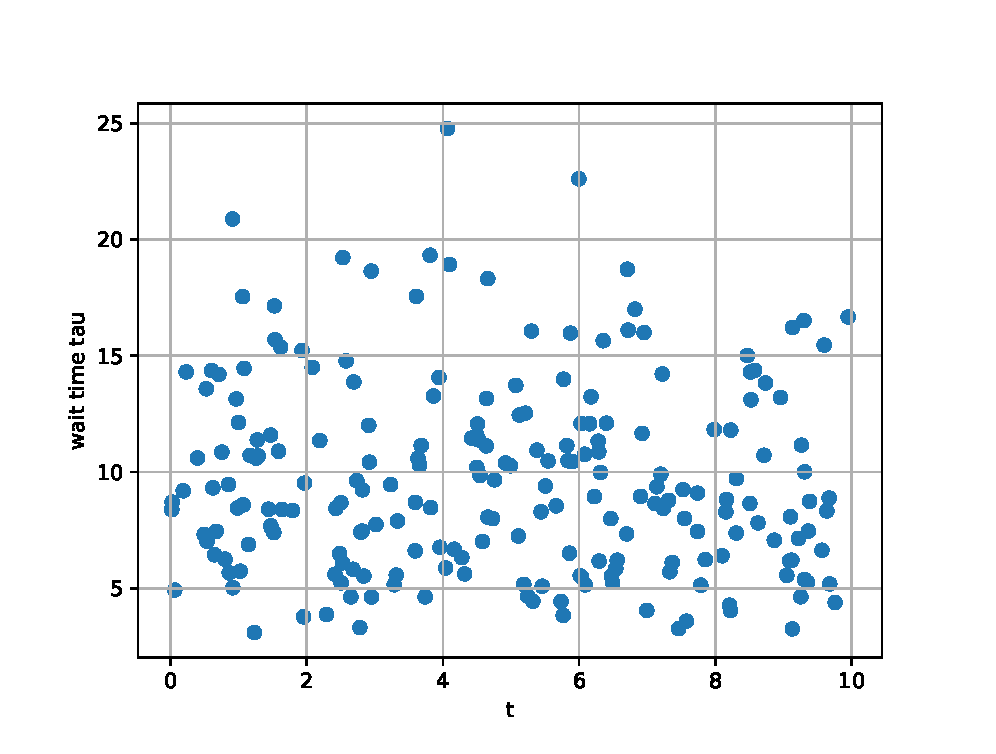
\includegraphics[width=1\textwidth]{data/ex11/SMO.eps}
\caption{Процесс с интенсивностью \(\lambda = 20\)}
\end{figure}

\subsubsection{Система массового обслуживания с циклической интенсивностью}

\begin{figure}[H]
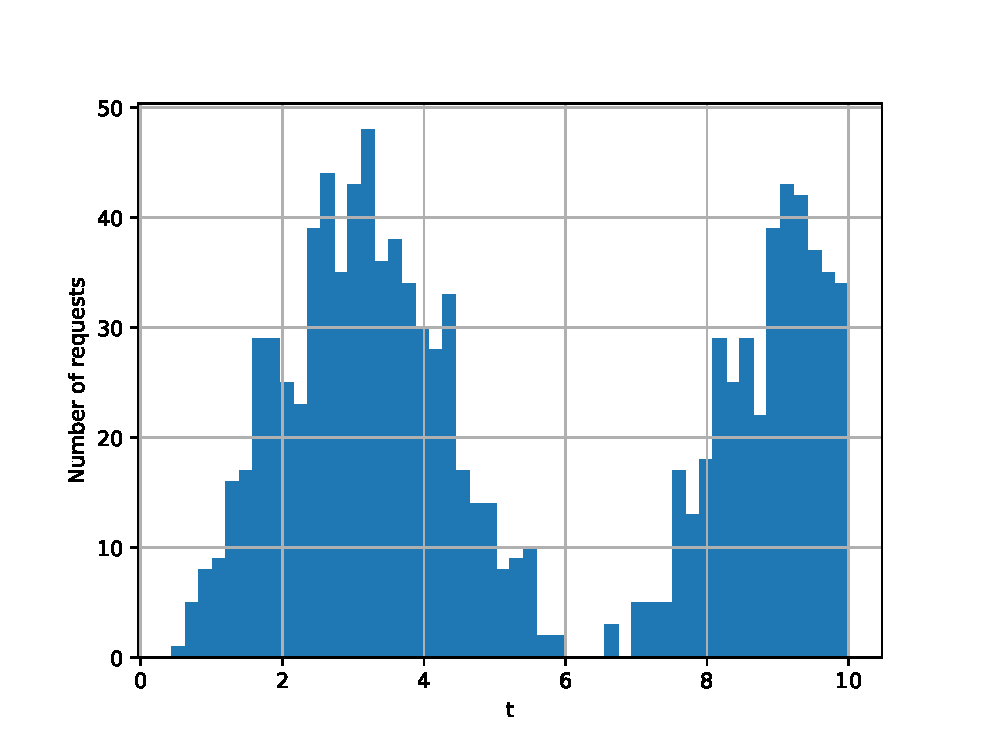
\includegraphics[width=1\textwidth]{data/ex11/cyclic.eps}
\caption{Процесс с интенсивностью \(\lambda_0 = 100\)}
\end{figure}

\subsubsection{Работа страховой компании}

\begin{figure}[H]
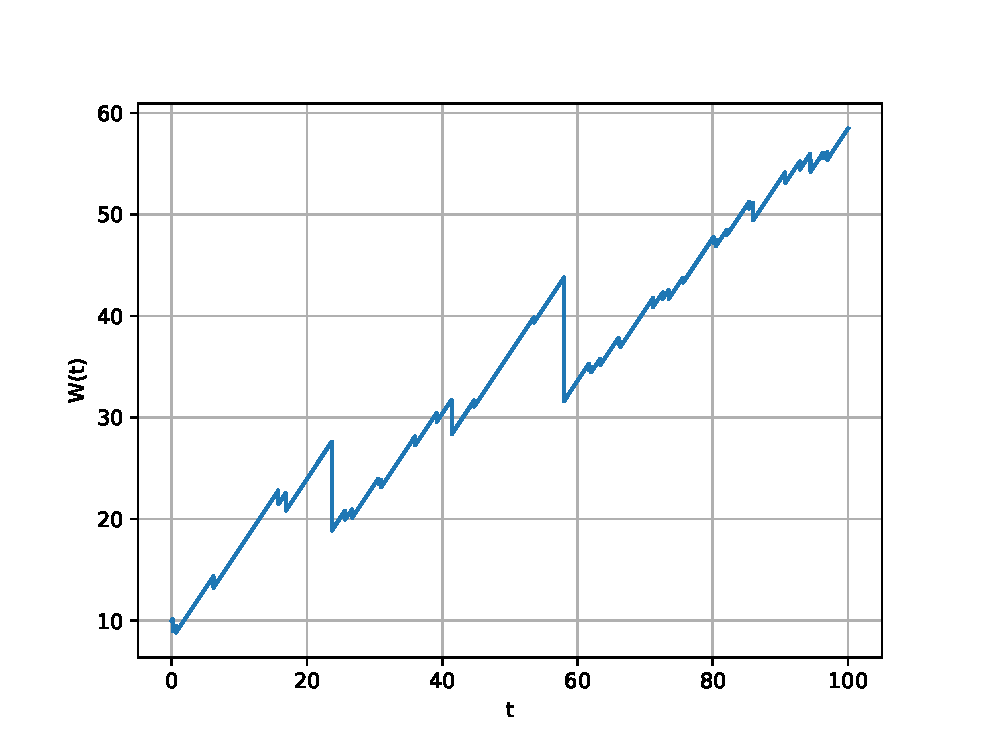
\includegraphics[width=1\textwidth]{data/ex11/pareto1.eps}
\caption{Пример 1. $x_m = 1/2,\, k = 2,\, \lambda = 1/2,\, c = 1.\ c - \lambda \frac{kx_m}{k - 1} = \frac{1}{2} > 0.$}
\end{figure}

\begin{figure}[H]
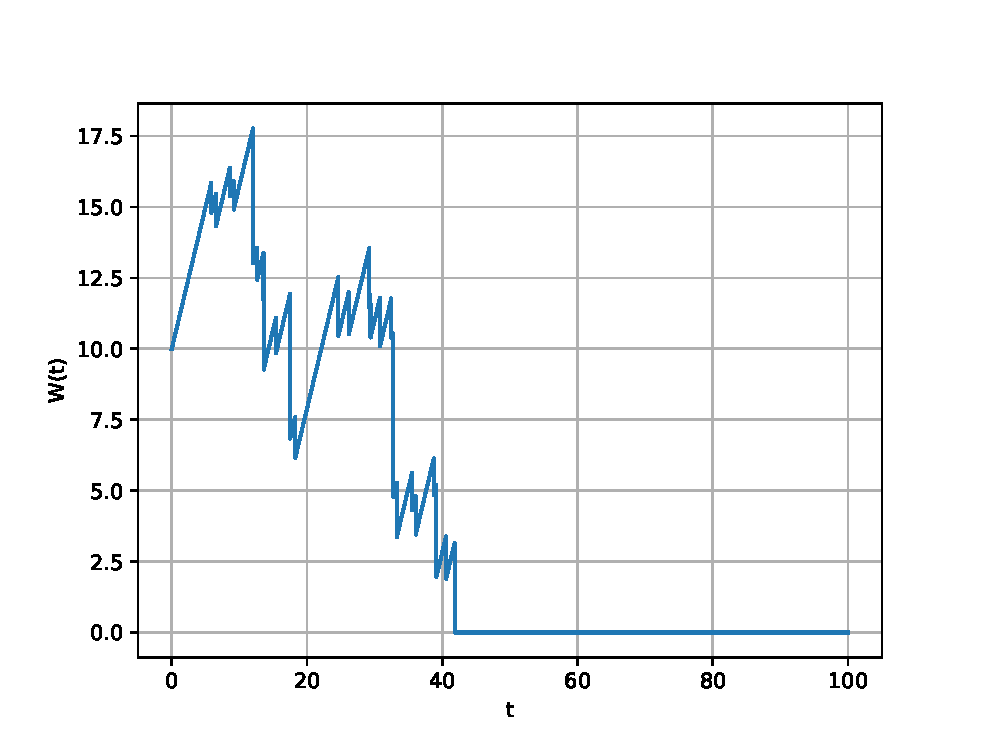
\includegraphics[width=1\textwidth]{data/ex11/pareto2.eps}
\caption{Пример 2. $x_m = 1,\, k = 2,\, \lambda = 0.6,\, c = 1.\ c - \lambda \frac{kx_m}{k - 1} = -1 < 0.$}
\end{figure}

\begin{figure}[H]
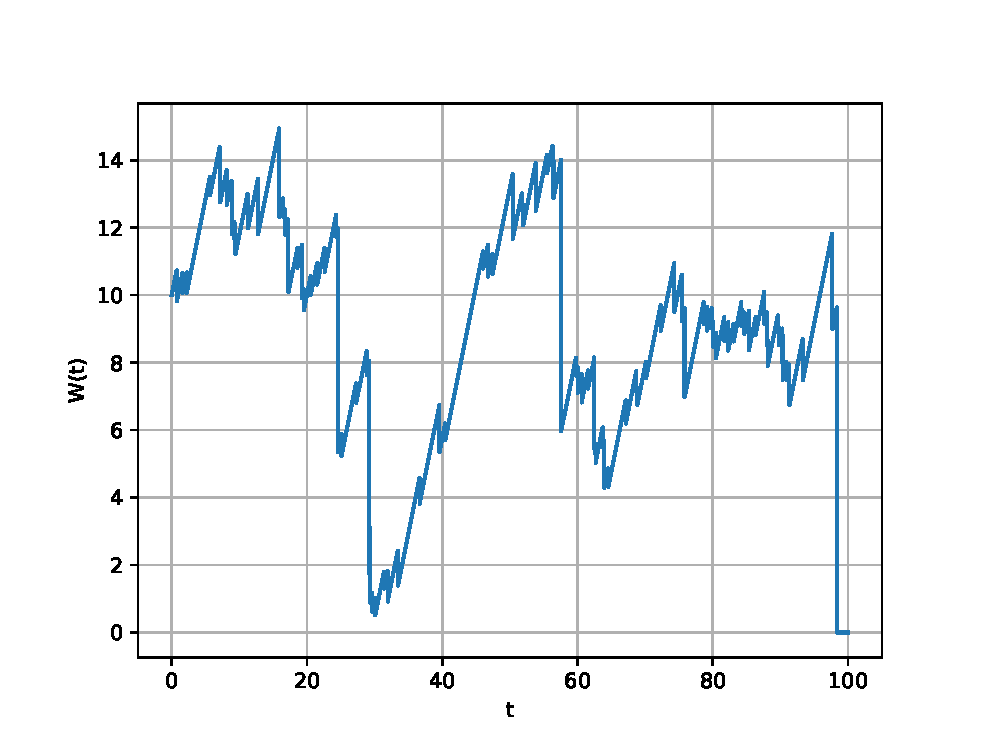
\includegraphics[width=1\textwidth]{data/ex11/pareto3.eps}
\caption{Пример 3. $x_m = 1/2,\, k = 2,\, \lambda = 1,\, c = 1.\ c - \lambda \frac{kx_m}{k - 1} = 0.$}
\end{figure}

\end{document}